% Chapter 4

\chapter{Metódy určenia ďalších parametrov štruktúry MOS.}\label{Chapter4}
\lhead{Kapitola 4. \emph{Metódy určenia ďalších parametrov štruktúry MOS}}
%- - - - - - - - - - - - - - - - - - - - - - - - - - - - - - - - - - - - -

V kapitole~\ref{Chapter3} sme popísali C-V metódy, ktoré budeme
používať na určovanie parametrov štruktúr MOS\@. Predovšetkým sa
budeme zaoberať určením koncentračného profilu dotujúcich prímesí v
podpovrchovej oblasti polovodiča, pretože niektoré metódy určovania
ďalších parametrov štruktúry MOS vychádzajú z predpokladu, že priebeh
koncentrácie je známy. Pri určovaní priebehov koncentračných profilov,
ktoré nie sú homogénne, sa používajú modely, ktorých presnosť
aproximácie daného fyzikálneho javu závisí od gradientu koncentrácie
prímesí~\cite{4.1, 4.2, 4.3, 4.4}. Aby sme overili presnosť použitých
aproximácií, vykonali sme porovnanie koncentračných profilov:

\begin{itemize}
\item použitého pri výpočte teoretickej C-V závislosti a
\item získaného z tejto teoretickej C-V závislosti~\cite{4.5}.
\end{itemize}

Výsledky sú uvedené v časti~\ref{sec:4.1.4}.

\par Ďalším parametrom, ktorý budeme určovať, je hustota pascí
rozhrania $Si-SiO_{2}$. Tu prichádzajú do úvahy dva
postupy. Porovnanie vysokofrekvenčnej a nízkofrekvenčnej C-V
závislosti, alebo porovnanie experimentálnej a teoretickej C-V
závislosti. Ich aplikácia je popísaná v časti~\ref{sec:4.2}.

\par Určenie generačného času života minoritných nosičov náboja, ktoré
súvisí s metódou konštantnej šírky OPN, bolo popísané v
časti~\ref{sec:3.4}.

\section[Určenie koncentračného profilu prímesí]{Určenie koncentračného profilu prímesí v podpovrchovej oblasti polovodiča.}\label{sec:4.1}

Problematika merania koncentračných profilov bola na našom oddelení
spracovaná v práci~\cite{4.6}. Tu sa budeme zaoberať len niektorými
aspektmi tejto problematiky, ktoré súvisia s určením nehomogénneho
koncentračného profilu prímesí v polovodiči.

\par Samostatné okruhy problémov pri určovaní koncentračného profilu
prímesí, ktorý označíme $N(x)$, tvoria:

\begin{itemize}
\item korekcia vypočítanej koncentrácie v oblasti od povrchu
  polovodiča do hĺbky $2L_{DE}$~\cite{4.7, 4.8}
\item určenie hĺbky vypočítanej koncentrácie, opierajúca sa o modely
  určenia šírky OPN~\cite{4.9, 4.10, 4.11}
\item korekcia vplyvu pascí rozhrania $Si-SiO_2$~\cite{4.12}
\item rozdiel medzi koncentráciou dotujúcich prímesí $N(x)$ a
  koncentráciou majoritných nosičov náboja $n(x)$.
\end{itemize}

Postupne sa budeme zaoberať uvedenými okruhmi problémov.

\subsection[Korekcia koncentrácie dotujúcich prímesí]{Korekcia koncentrácie dotujúcich prímesí pri povrchu polovodiča.}\label{sec:4.1.1}

Známy vzťah pre výpočet $N(x)$~\cite{I.2}

\begin{equation}\label{eq:4.1}
  N(x) = {\frac{2}{q\epsilon}} {\Bigg[\frac{dC_{sc}^{-2}}{d\varphi_{s}}\Bigg]}^{-1}
\end{equation}

bol odvodený z riešenia Poissonovej rovnice s použitím aproximácie
hlbokého ochudobnenia. Táto aproximácia neplatí pre šírku OPN menšiu
ako $2L_{DE}$.  Aby sme dosiahli správne výsledky aj v tejto oblasti,
musíme $N(x)$ vypočítané podľa~\ref{eq:4.1} korigovať postupom
odvodeným v~\cite{4.7, 4.8}. Z práce~\cite{4.7} je zrejmý aj
fyzikálny význam tejto korekcie, ktorá je funkciou povrchového
potenciálu

\begin{equation}\label{eq:4.2}
  {N(x)}_{korigovane} = N(x)f(\varphi_{s})
\end{equation}

, kde

\begin{equation}\label{eq:4.3}
  f(\varphi_{s}) = {\frac{1}{1-e^{-\beta\varphi_{s}}}} - {\frac{2e^{-\beta\varphi_{s}}\big[e^{-\beta\varphi_{s}}+\beta\varphi_{s} - 1\big]}{\big[1 - e^{-\beta\varphi_{s}}\big]}} \qquad,kde\quad \beta=\frac{q}{kT}
\end{equation}

Povrchový potenciál, použitý vo vzťahu~\ref{eq:4.3} možno určiť
podla~\cite{4.7} numerickým riešením rovnice

\begin{equation}\label{eq:4.4}
  \frac{C_{sc}^{2}}{\varphi_{s}}\frac{C_{sc}^{-2}}{d\varphi_{s}}=\frac{1-e^{-\beta\varphi_{s}}}{e^{-\beta\varphi_{s}}+\beta\varphi_{s}-1}-\frac{2e^{-\beta\varphi_{s}}} {1-e^{-\beta\varphi_{s}}}
\end{equation}

Tu treba poznamenať, že vzťah~\ref{eq:4.4} bol odvodený pomocou vzťahu
pre kapacitu OPN $C_{sc}$, ktorý predpokladá homogénnu koncentráciu
prímesí. Pretože experimentálne zistená diferenciálna kapacita
$C_{sc}$ závisí od zmeny náboja na hranici OPN (čo využíva
vzťah~\ref{eq:4.1}), bude povrchový potenciál získaný zo
vzťahu~\ref{eq:4.4} predstavovať potenciál, ktorý by bol na povrchu
polovodiča, ak by koncentrácia $N(x)$ v celej oblasti OPN bola
konštantná a zároveň rovná koncentrácii na hranici OPN (ktorú určujeme
podľa~\ref{eq:4.1}). Z uvedeného vyplýva, že pre nehomogénne dotované
substráty pomocou vzťahu~\ref{eq:4.4} nemožno získať skutočný priebeh
$\varphi_{s}(V_{g})$, napriek tomu, že korekcia~\ref{eq:4.2} dáva
dobré výsledky aj v tomto prípade.

\subsection[Určenie hĺbky koncentračného profilu.]{Určenie hĺbky koncentračného profilu.}\label{sec:4.1.2}

Po určení koncentrácie podľa vzťahu~\ref{eq:4.2} treba zároveň určiť
polohu vypočítanej koncentrácie. Bežne používaný vzťah vychádzajúci z
modelu doskového kondenzátora (čo predstavuje aproximáciu hlbokého
ochudobnenia)

\begin{equation}\label{eq:4.5}
  w(C_{sc})=\frac{\epsilon}{C_{sc}}
\end{equation}

neplatí pre hĺbky menšie ako $2L_{DE}$. V tejto oblasti možno použiť
vzťah odvodený pomocou aproximácie priebehu potenciálu v polovodiči
$\varphi(x)$. Uvedená problematika bola na našom oddelení podrobne
spracovaná v~\cite{4.13, 4.14}, keď boli použité výsledky
prác~\cite{4.9, 4.10, 4.11}. Pre výpočet hĺbky v tejto oblasti môžeme
použiť vzťah, ktorý predstavuje aproximáciu priebehu potenciálu v
polovodiči $\varphi(x)$~\cite{I.1}

\begin{equation}\label{eq:4.6}
  w(\varphi_{s})=\sqrt{2}L_{DE}{\big[e^{-\beta\varphi_{s}}+\beta\varphi_{s}-1\big]}^{\frac{1}{2}}
\end{equation}

, kde 

\begin{equation}\label{eq:4.7}
  L_{DE} = {\Big[\frac{\epsilon}{\beta qN}\Big]}^{\frac{1}{2}}
\end{equation}

je extrinzická Debayova dĺžka, pri výpočte ktorej sme použili
koncentráciu získanú zo vzťahu~\ref{eq:4.2}.  Vo vzťahu~\ref{eq:4.6}
použijeme hodnotu $\varphi_{s}$ získanú z riešenia
vzťahu~\ref{eq:4.4}.  Napriek tomu, že aj vzťah~\ref{eq:4.6} bol
odvodený za predpokladu homogénneho rozloženia prímesí v polovodiči,
jeho použitie v spojení s riešení rovnice~\ref{eq:4.4} dáva uspokojivé
výsledky, ako ukážeme neskôr.

\begin{figure}[h!]\centering
  \begin{minipage}[c]{\myfiguresize}
    \begin{center}
      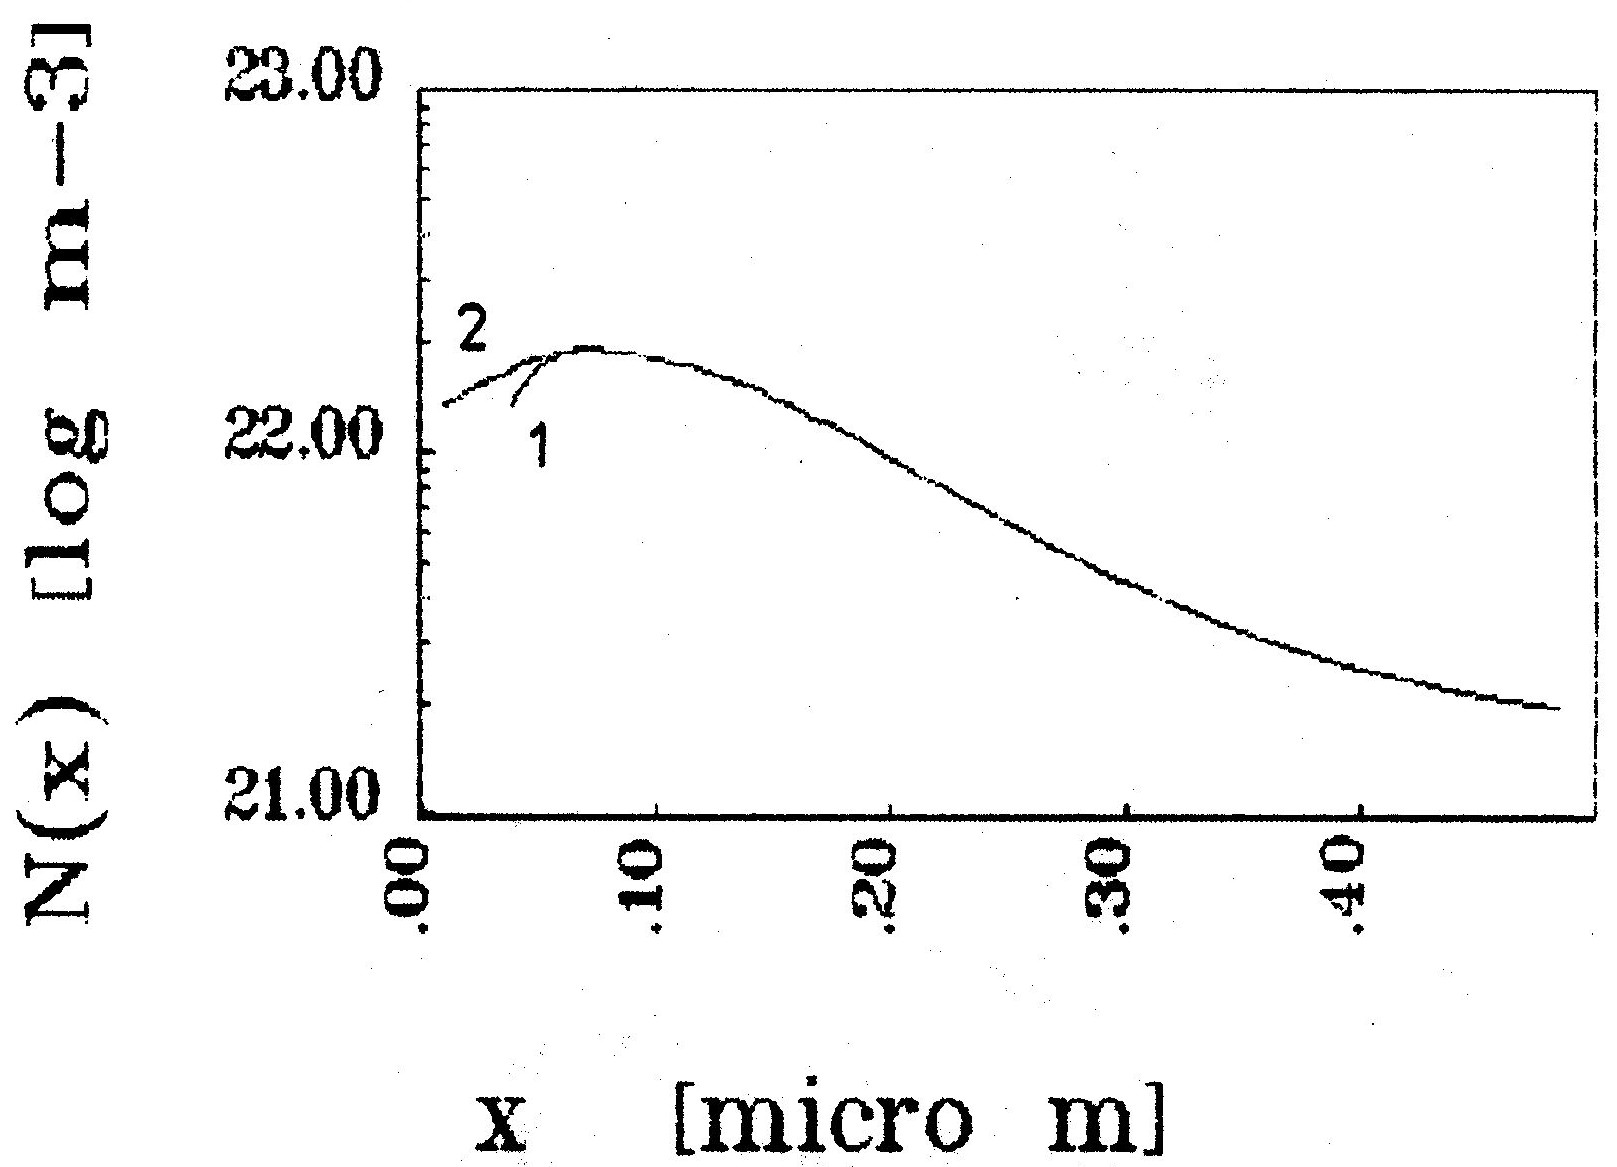
\includegraphics{Figures/fig-4-1.eps}% chktex-file 8
      \caption[Priebeh koncentrácie dotujúcich prímesí v polovodiči
        vypočítaný zo vzťahu~\ref{eq:4.2}]{Priebeh koncentrácie
        dotujúcich prímesí v polovodiči vypočítaný zo
        vzťahu~\ref{eq:4.2}. Vzdialenosť od povrchu bola určená zo
        vzťahov~\ref{eq:4.5} (krivka 1) a~\ref{eq:4.6} (krivka
        2).}\label{fig:4.1}
    \end{center}
  \end{minipage}
\end{figure}
% OBR26.BIT

Na obrázku~\ref{fig:4.1} sú znázornené priebehy $N(x)$ s použitím
korekcie~\ref{eq:4.2}, prezentujúce rozdiel v použití
vzťahov~\ref{eq:4.5} a~\ref{eq:4.6}. Tu je zrejmé, že použitím
vzťahu~\ref{eq:4.6} možno vypočítať priebeh koncentrácie dotujúcich
prímesí bližšie k povrchu polovodiča, čo má význam pre ďalšie výpočty,
ktoré predpokladajú znalosť priebehu $N(x)$.

Prvý stĺpec tabuľky~\ref{tab:4.1} obsahuje hodnoty $\varphi_{s}$
určené riešením rovnice~\ref{eq:4.4} a v druhom stĺpci sa nachádzajú
hodnoty korekčného faktora~\ref{eq:4.3}. Ďalšie dva stĺpce umožňujú
porovnanie nekorigovanej a korigovanej hodnoty $N(x)$ a v posledných
dvoch stĺpcoch sú uvedené hodnoty $w(\varphi_{s})$ a $w(C_{sc})$
získané zo vzťahov~\ref{eq:4.5} a~\ref{eq:4.6}.

\begin{table}[h!]\centering
  \begin{minipage}[c]{\myfiguresize}
    \begin{center}
      \begin{tabular}{c c c c c c}
      $\varphi_{s}[V]$ & $f(\varphi_{s})$ & $N[m^{-3}]$ & $N_{kor.}[m^{-3}]$ & $w(\varphi_{s})[\mu m]$ & $w(C_{SC})[\mu m]$ \\
      \hline% chktex-file 44
      0.007 & 0.39 & $0.35\times10^{23}$ & $0.14\times10^{23}$ & 0.0102 & 0.0389 \\
      0.016 & 0.44 & $0.33\times10^{23}$ & $0.15\times10^{23}$ & 0.0190 & 0.0413 \\
      0.024 & 0.50 & $0.31\times10^{23}$ & $0.15\times10^{23}$ & 0.0265 & 0.0438 \\
      0.032 & 0.56 & $0.29\times10^{23}$ & $0.16\times10^{23}$ & 0.0333 & 0.0466 \\
      0.041 & 0.61 & $0.28\times10^{23}$ & $0.17\times10^{23}$ & 0.0391 & 0.0494 \\
      0.049 & 0.66 & $0.27\times10^{23}$ & $0.18\times10^{23}$ & 0.0444 & 0.0523 \\
      0.057 & 0.71 & $0.26\times10^{23}$ & $0.18\times10^{23}$ & 0.0493 & 0.0553 \\
      0.065 & 0.76 & $0.25\times10^{23}$ & $0.19\times10^{23}$ & 0.0538 & 0.0585 \\
      0.073 & 0.80 & $0.24\times10^{23}$ & $0.19\times10^{23}$ & 0.0581 & 0.0617 \\
      0.081 & 0.83 & $0.23\times10^{23}$ & $0.19\times10^{23}$ & 0.0623 & 0.0650 \\
      0.090 & 0.86 & $0.22\times10^{23}$ & $0.19\times10^{23}$ & 0.0664 & 0.0684 \\
      0.098 & 0.89 & $0.22\times10^{23}$ & $0.19\times10^{23}$ & 0.0704 & 0.0719 \\
      0.106 & 0.91 & $0.21\times10^{23}$ & $0.19\times10^{23}$ & 0.0743 & 0.0755 \\
      0.115 & 0.93 & $0.21\times10^{23}$ & $0.19\times10^{23}$ & 0.0783 & 0.0791 \\
      0.124 & 0.94 & $0.20\times10^{23}$ & $0.19\times10^{23}$ & 0.0822 & 0.0828 \\
      0.133 & 0.96 & $0.20\times10^{23}$ & $0.19\times10^{23}$ & 0.0861 & 0.0866 \\
      0.142 & 0.97 & $0.19\times10^{23}$ & $0.19\times10^{23}$ & 0.0900 & 0.0904 \\
      0.151 & 0.97 & $0.19\times10^{23}$ & $0.18\times10^{23}$ & 0.0939 & 0.0942 \\
      0.160 & 0.98 & $0.19\times10^{23}$ & $0.18\times10^{23}$ & 0.0978 & 0.0981 \\
      0.169 & 0.99 & $0.18\times10^{23}$ & $0.18\times10^{23}$ & 0.1018 & 0.1019 \\
      0.178 & 0.99 & $0.18\times10^{23}$ & $0.18\times10^{23}$ & 0.1058 & 0.1058 \\
      0.187 & 0.99 & $0.18\times10^{23}$ & $0.17\times10^{23}$ & 0.1098 & 0.1098 \\
      0.205 & 1.00 & $0.17\times10^{23}$ & $0.17\times10^{23}$ & 0.1179 & 0.1179 \\
      \end{tabular}
      \caption[Výpočet koncentračného profilu prímesí $N(x)$]{Výpočet
        koncentračného profilu prímesí $N(x)$.}\label{tab:4.1}
    \end{center}
  \end{minipage}
\end{table}

\begin{minipage}[c]{\textwidth}
  \emph{POZNÁMKA.} Pomocou aproximácie~\ref{eq:4.6}, ktorá predstavuje
  šírku OPN ako funkciu povrchového potenciálu polovodiča
  (koncentrácia je parameter), možno aproximovať priebeh $\varphi(x)$
  pre danú šírku OPN aj v prípade, že substrát polovodiča je
  nehomogénne dotovaný.  Vlastný postup určenia koncentrácie
  dotujúcich prímesí z kapacitného merania predstavuje diskretizáciu
  spojitého priebehu $N(x)$, kde jednotlivé hodnoty $N_i$ predstavujú
  aproximáciu koncentrácie v oblasti hranice OPN~\cite{4.1, 4.2, 4.3}.
  Úbytok potenciálu $\Delta\varphi_i$ na vrstve šírky $\Delta
  w_{i}=w_{i+1}-w_{i}$ s koncentráciou $N_i$ možno určiť riešením
  vzťahu
  \begin{equation}\label{eq:4.8}
    \Delta w_{i} = \sqrt{2}L_{DE_{i}}{\Big[e^{-\beta\Delta\varphi_{i}} + \beta\Delta\varphi_{i} - 1\Big]}^{\frac{1}{2}}
  \end{equation}
  , kde% chktex-file 26
  \begin{equation}\label{eq:4.9}
    L_{DE_{i}} = {\bigg[\frac{\epsilon}{\beta qN_{i}}\bigg]}^{\frac{1}{2}}
  \end{equation}
  Potom priebeh $\varphi(x)$ možno získať použitím
  vzťahov~\ref{eq:4.8} a~\ref{eq:4.9} ak s výpočtom začneme od hranice
  OPN, kde predpokladáme potenciál rovný nule, smerom k povrchu
  polovodiča.
\end{minipage}

\subsection[Vplyv pascí rozhrania $Si-SiO_{2}$ a generácie minoritných nosičov náboja.]{Vplyv pascí rozhrania $Si-SiO_{2}$ a generácie minoritných nosičov náboja}\label{sec:4.1.3}

V oblasti inverzie dochádza v OPN ku generácii minoritných nosičov
náboja, ktoré vytvárajú inverznú vrstvu a ovplyvňujú veľkosť kapacity
štruktúry MOS\@. Aby sme namerali C-V závislosť v oblasti hlbokého
ochudobnenia, ktorá nie je ovplyvnená minoritnými nosičmi náboja,
použijeme impulznú HF C-V metódu. Namerané hodnoty $N(x)$ získané
pomocou tejto metódy sú na obrázku~\ref{fig:4.2}.

\begin{figure}[h!]\centering
  \begin{minipage}[c]{\myfiguresize}
    \begin{center}
      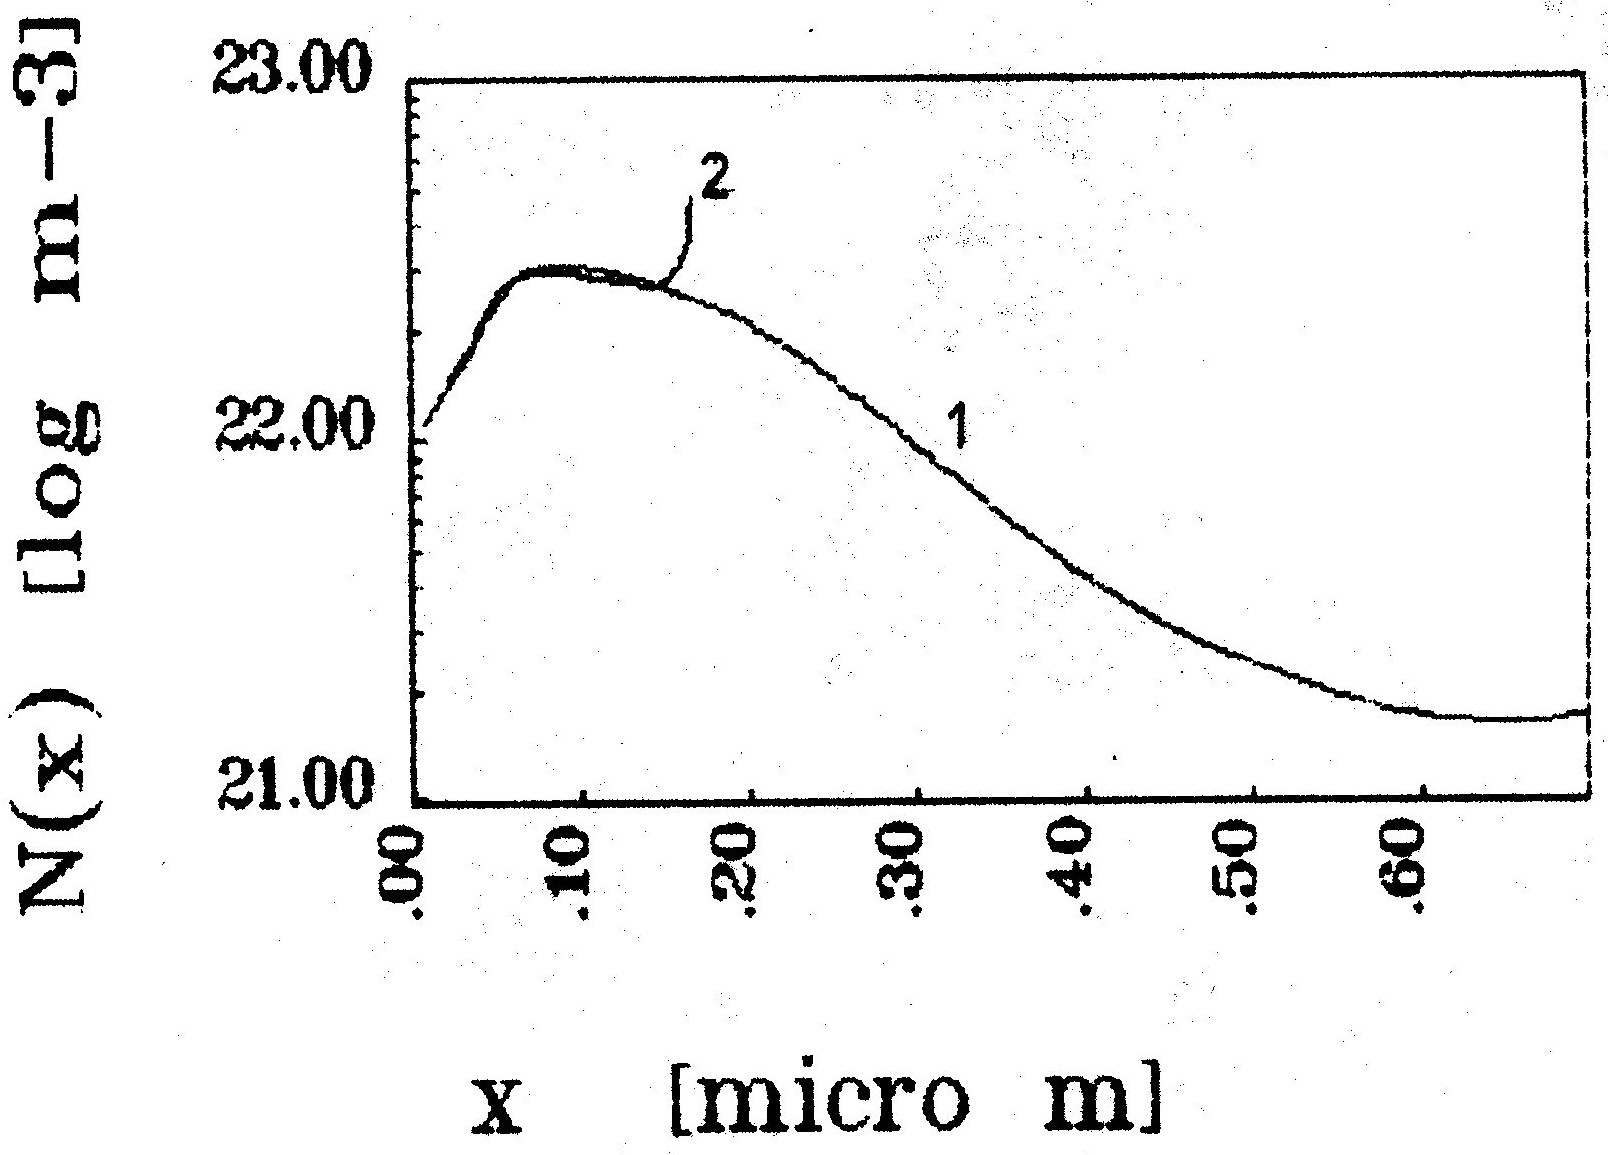
\includegraphics{Figures/fig-4-2.eps}% chktex-file 8
      \caption[Priebeh koncentračného profilu dotujúcich prímesí
        získaný z C-V závislosti v oblasti hlbokého ochudobnenia a z
        rovnovážnej C-V závislosti]{Priebeh koncentračného profilu
        dotujúcich prímesí získaný z C-V závislosti v oblasti hlbokého
        ochudobnenia (krivka 1) a z rovnovážnej C-V závislosti (krivka
        2). Pre výpočet závislosti $N(x)$ boli použité C-V závislosti
        zobrazené na obrázku~\ref{fig:3.2}}\label{fig:4.2}
    \end{center}
  \end{minipage}
\end{figure}
% OBR8.BIT

\par Pri výpočte $N(x)$ pomocou
vzťahov~\ref{eq:4.1},~\ref{eq:4.2},~\ref{eq:4.3},~\ref{eq:4.4}
a~\ref{eq:4.6} sa používa aproximácia

\begin{equation}\label{eq:4.10}
  \frac{dC_{sc}^{-2}}{d\varphi_{s}} \cong \frac{dC_{mos}^{-2}}{dV_{g}}
\end{equation}

kde rovnosť platí v prípade, že hustota pascí rozhrania $Si-SiO_{2}$
je rovná nule. Nameraná HF C-V závislosť je však vždy do určitej miery
ovplyvnená pascami rozhrania, ktoré počas merania menia svoj
stav~\cite{4.15}. Tento vplyv možno zmenšovať zvyšovaním frekvencie
meracieho signálu a rýchlejším meraním kapacity po napäťovom skoku
impulznej C-V metódy.  Problému použitia aproximácie~\ref{eq:4.10} sa
vyhneme, ak použijeme na určenie $N(x)$ dáta namerané pomocou Q-C
metódy, pri ktorej vieme určiť priebeh povrchového potenciálu
$\varphi_{s}(V_{g})$.

\par Ak určujeme koncentračný profil dotujúcich prímesí z HF C-V
závislosti, môžeme vplyv pascí rozhrania $Si-SiO_{2}$ korigovať v
oblasti ochudobnenia vzťahom uvedeným v~\cite{I.1}

\begin{equation}\label{eq:4.11}
  {N(x)}_{korigovane} = {N(x)}{\cfrac{1-\cfrac{C_{mos}^{LF}}{C_{ox}}}{1-\cfrac{C_{mos}^{HF}}{C_{ox}}}}
\end{equation}

za predpokladu, že poznáme priebeh nízkofrekvenčnej C-V závislosti.


\subsection[Výpočet koncentračného profilu dotujúcich prímesí z priebehu majoritných nosičov náboja a overenie použitých modelov.]{Výpočet koncentračného profilu dotujúcich prímesí z priebehu majoritných nosičov náboja a overenie použitých modelov.}\label{sec:4.1.4}

Ako vidieť z obrázku~\ref{fig:1.1}, pre nehomogénny priebeh
koncentrácie dotujúcich atómov dochádza v dôsledku difúzie majoritných
nosičov náboja k rozdielu medzi uvedenými priebehmi~\cite{4.16}. Je
známe~\cite{4.17}, že pomocou vzťahu~\ref{eq:4.1} určujeme priebeh
koncentrácie majoritných nosičov náboja namiesto koncentrácie
dotujúcich prímesí. V práci~\cite{4.18} je popísaná korekcia, pomocou
ktorej možno určiť presný priebeh koncentrácie dotujúcich atómov z
nameraného priebehu $n(x)$ (ak nameraný priebeh $n(x)$ skutočne
predstavuje priebeh majoritných nosičov náboja).

\begin{figure}[h!]\centering
  \begin{minipage}[c]{\myfiguresize}
    \begin{center}
      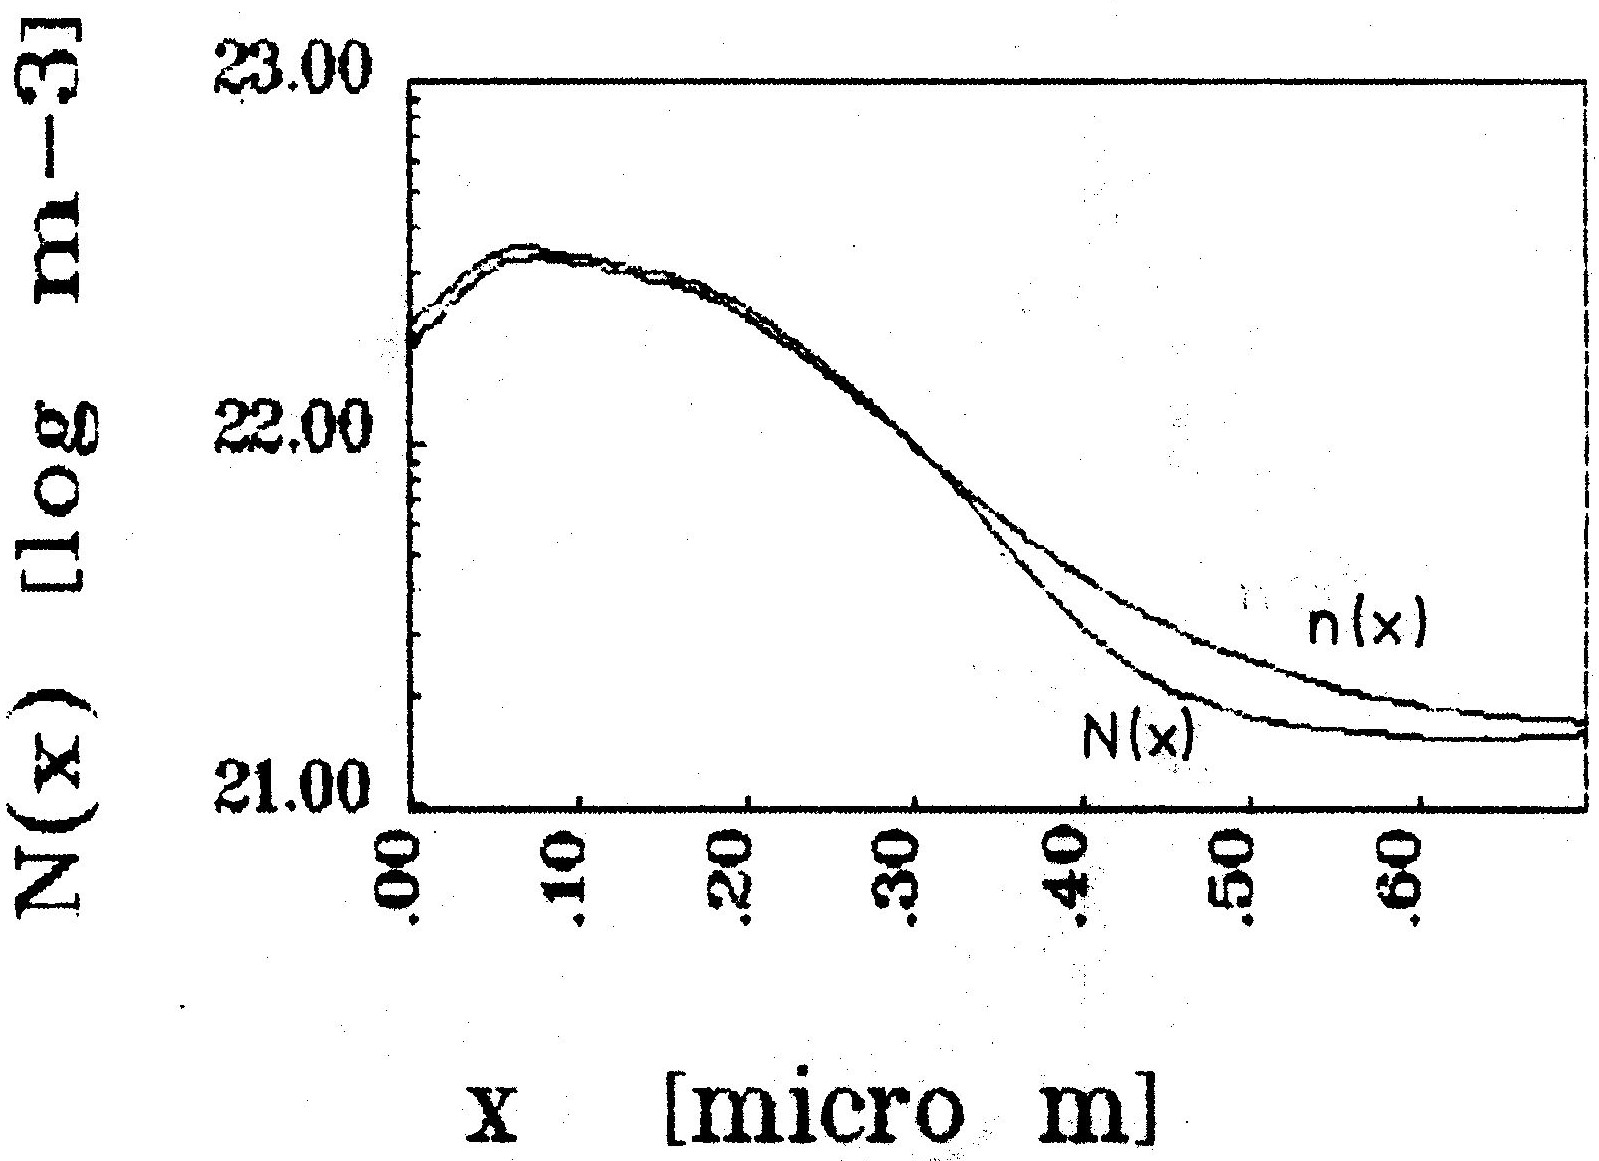
\includegraphics{Figures/fig-4-3.eps}
      \caption[Priebeh koncentrácie majoritných nosičov náboja $n(x)$
        určený z ochudobnenej HF C-V závislosti a priebeh dotujúcich
        atómov $N(x)$ určený zo vzťahu~\ref{eq:4.12}]{Priebeh
        koncentrácie majoritných nosičov náboja $n(x)$ určený z
        ochudobnenej HF C-V závislosti a priebeh dotujúcich atómov
        $N(x)$ určený zo vzťahu~\ref{eq:4.12}.}\label{fig:4.3}
    \end{center}
  \end{minipage}
\end{figure}
% OBR23.BIT

\begin{equation}\label{eq:4.12}
  N(x) = n(x) - {\frac{kT\epsilon}{q^{2}} {\frac{d}{dx}} {\Bigg[\frac{1}{n(x)}\frac{dn(x)}{dx}\Bigg]}}
\end{equation}

Na obrázku~\ref{fig:4.3} sú znázornené priebehy $n(x)$ a $N(x)$. Vo
vzťahu~\ref{eq:4.12} vystupuje druhá derivácia $n(x)$, ktorú v prípade
experimentálnych hodnôt $n(x)$ musíme určiť numericky.

\par Určovanie derivácie empiricky získanej funkčnej závislosti je
problém, s ktorým sa možno často stretnúť pri spracovaní nameraných
dát. V základných kurzoch numerickej matematiky~\cite{4.19} sa
dokazuje, že diferenciácia zosilňuje šum spracovávaných dát. Pritom
šumom tu všeobecne označujeme odchýlku spracovávaných dát od ich
skutočnej hodnoty, ktorá môže vzniknúť dôsledkom:

\begin{itemize}
\item fyzikálnych javov
\item chyby meracieho prístroja
\item zaokrúhľovania pri číslicovom spracovaní.
\end{itemize}

\par To znamená, že frekvenčné spektrum spracovávaného signálu,
získané pomocou Fourierovej transformácie, bude obsahovať zložky,
ktoré je potrebné odstrániť pred (,alebo pri) výpočte derivácie. V
ďalšom budeme hovoriť o aproximácii pomocou polynómov, ktorá sa
používa najčastejšie, aj keď uvedené tvrdenia platia tiež pre iné
triedy funkcií.

\par Ak pre výpočet derivácie použijeme polynomiálne aproximácie, je
vhodné najprv funkčné hodnoty `vyhladiť'~\cite{4.20}. Pre potlačenie
šumu sú potom dôležité frekvenčné vlastnosti použitých numerických
metód, ktoré možno vyjadriť pomocou prenosovej charakteristiky. Týmto
prístupom môžeme porovnávať frekvenčné vlastnosti polynomiálnych
aproximácií a číslicových filtrov~\cite{4.21}.  Základným rozdielom
medzi výpočtom koeficientov číslicových filtrov a koeficientov
polynomiálnych aproximácií je, že v prvom prípade vychádzame z
požadovanej prenosovej charakteristiky a v druhom prípade sú
koeficienty počítané z podmienky najmenších štvorcov vzdialenosti
spracovávaných dát a polynómu daného stupňa. Z uvedeného vyplývajú
nedostatky polynomiálnych aproximácií:

\begin{itemize}
\item spracovávaná funkčná závislosť nemusí byť polynóm, aj keď
  existuje polynóm, ktorý interpoluje namerané hodnoty
\item frekvenčné vlastnosti metódy sú sekundárnym dôsledkom stupňa
  použitého polynómu a počtu bodov, cez ktoré sa tento polynóm
  prekladá.
\end{itemize}

\par Pretože v našom prípade spracovávame funkčné závislosti, ktoré
nie sú vo všeobecnosti polynómy, rozhodli sme sa pre použitie
číslicových filtrov. Tu možno ešte spomenúť, že pre úspešnú aplikáciu
číslicových filtrov je dôležité navrhnúť kritickú frekvenciu a veľkosť
filtra tak, aby filter neovplyvňoval amplitúdu signálu v tej časti
spektra, ktorá predstavuje užitočný signál. Pre určenie derivácií vo
vzorci~\ref{eq:4.12} sme použili nerekurzívny diferencujúci
dolnopriepustný číslicový filter, ktorého kritická frekvencia je
$f_{c}=0.1$ a jeho veľkosť je $2n+1=11$.

\par Je známe~\cite{4.18}, že aj priebeh $n(x)$, určený z nameranej
C-V závislosti, je zaťažený chybou, ak predstavuje nehomogénny
koncentračný profil. Presnejšie možno tvrdiť~\cite{4.3}, že zmeraná
koncentrácia $n(x)$ predstavuje priemernú hodnotu koncentrácie
majoritných nosičov v oblasti s dĺžkou rádove niekoľko $L_{DE}$. Potom
je otázkou, kedy ešte možno použiť aproximácie popísané v
častiach~\ref{sec:4.1},~\ref{sec:4.2} a s akou chybou.

\par V práci~\cite{4.22} sú popísané výsledky výpočtového experimentu,
kedy na základe experimentálne určeného profilu $N(x)$ bola vypočítaná
teoretická ochudobnená C-V krivka a porovnaná s nameranou C-V
krivkou. V prípade, že sa experimentálna a teoretická C-V závislosť
zhoduje, možno tvrdiť, ze $N(x)$ predstavuje skutočné rozdelenie
dotujúcich prímesí v polovodiči.

\par Nezávisle na~\cite{4.22} sme uskutočnili experiment, ktorého
výsledky uvedieme. Na obrázkoch~\ref{fig:4.4} a~\ref{fig:4.5} sú
znázornené priebehy $N(x)$, ktoré boli použité pri výpočte teoretickej
C-V závislosti. Pri riešení Poissonovej rovnice sme zároveň získali
priebeh koncentrácie majoritných nosičov náboja $n_{1}(x)$ pre
$V_{g}=0$, ktorý sa v dôsledku difúzie líši od priebehu koncentrácie
atómov $N(x)$. Z teoretických C-V závislostí boli pomocou
aproximácií~\ref{eq:4.2} a~\ref{eq:4.6} vypočítané priebehy
$n_{2}(x)$.  Porovnávali sme závislosti $n(x)$, pretože zhoda
koncentrácie majoritných nosičov náboja znamená aj zhodu priebehu
koncentrácie dotujúcich atómov.

\par Ako vidieť na obrázku~\ref{fig:4.4}, pre tento koncentračný
profil je použitie kapacitnej metódy vhodné, zatiaľ čo v prípade
zobrazenom na obrázku~\ref{fig:4.5} je zrejmý veľký rozdiel medzi
skutočným $n_{1}(x)$ a nameraným priebehom $n_{2}(x)$.

\begin{figure}[h!]\centering
  \begin{minipage}[c]{\myfiguresize}
    \begin{center}
      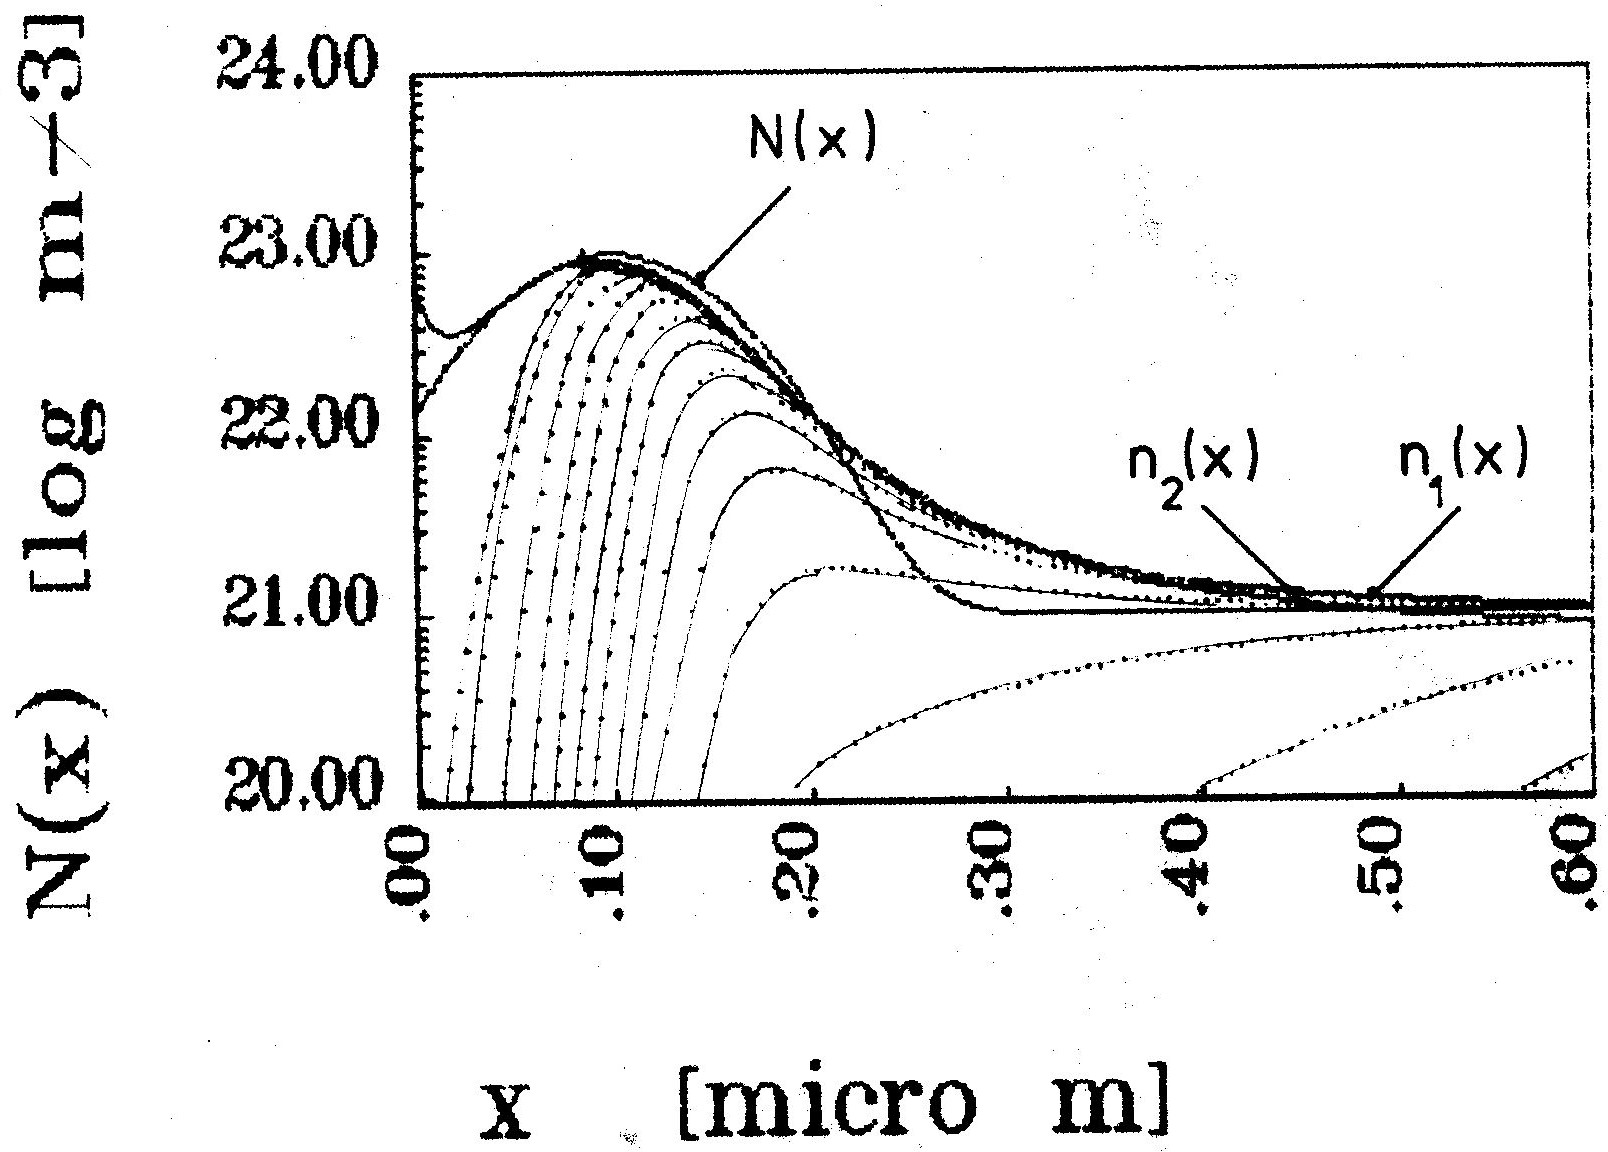
\includegraphics{Figures/fig-4-4.eps}
      \caption[Priebeh koncentrácie prímesí simulovaný Gaussovským
        rozložením]{Priebeh koncentrácie prímesí $N(x)$ simulovaný
        Gaussovským rozložením s parametrami $R_{p}=0.1\mu m$, $\Delta
        R_{p}=0.05\mu m$, $N_{\max}=1.0\times 10^{23} m^{-3}$,
        $N_{bulk}=1.0\times10^{21}m^{-3}$; priebeh majoritných nosičov
        náboja $n_{1}(x)$ a priebeh $n_{2}(x)$, získaný z teoretickej
        C-V závislosti. Bodkovanými čiarami je znázornené
        ochudobňovanie štruktúry MOS.}\label{fig:4.4}
    \end{center}
  \end{minipage}
\end{figure}
% OBR24.BIT

\begin{figure}[h!]\centering
  \begin{minipage}[c]{\myfiguresize}
    \begin{center}
      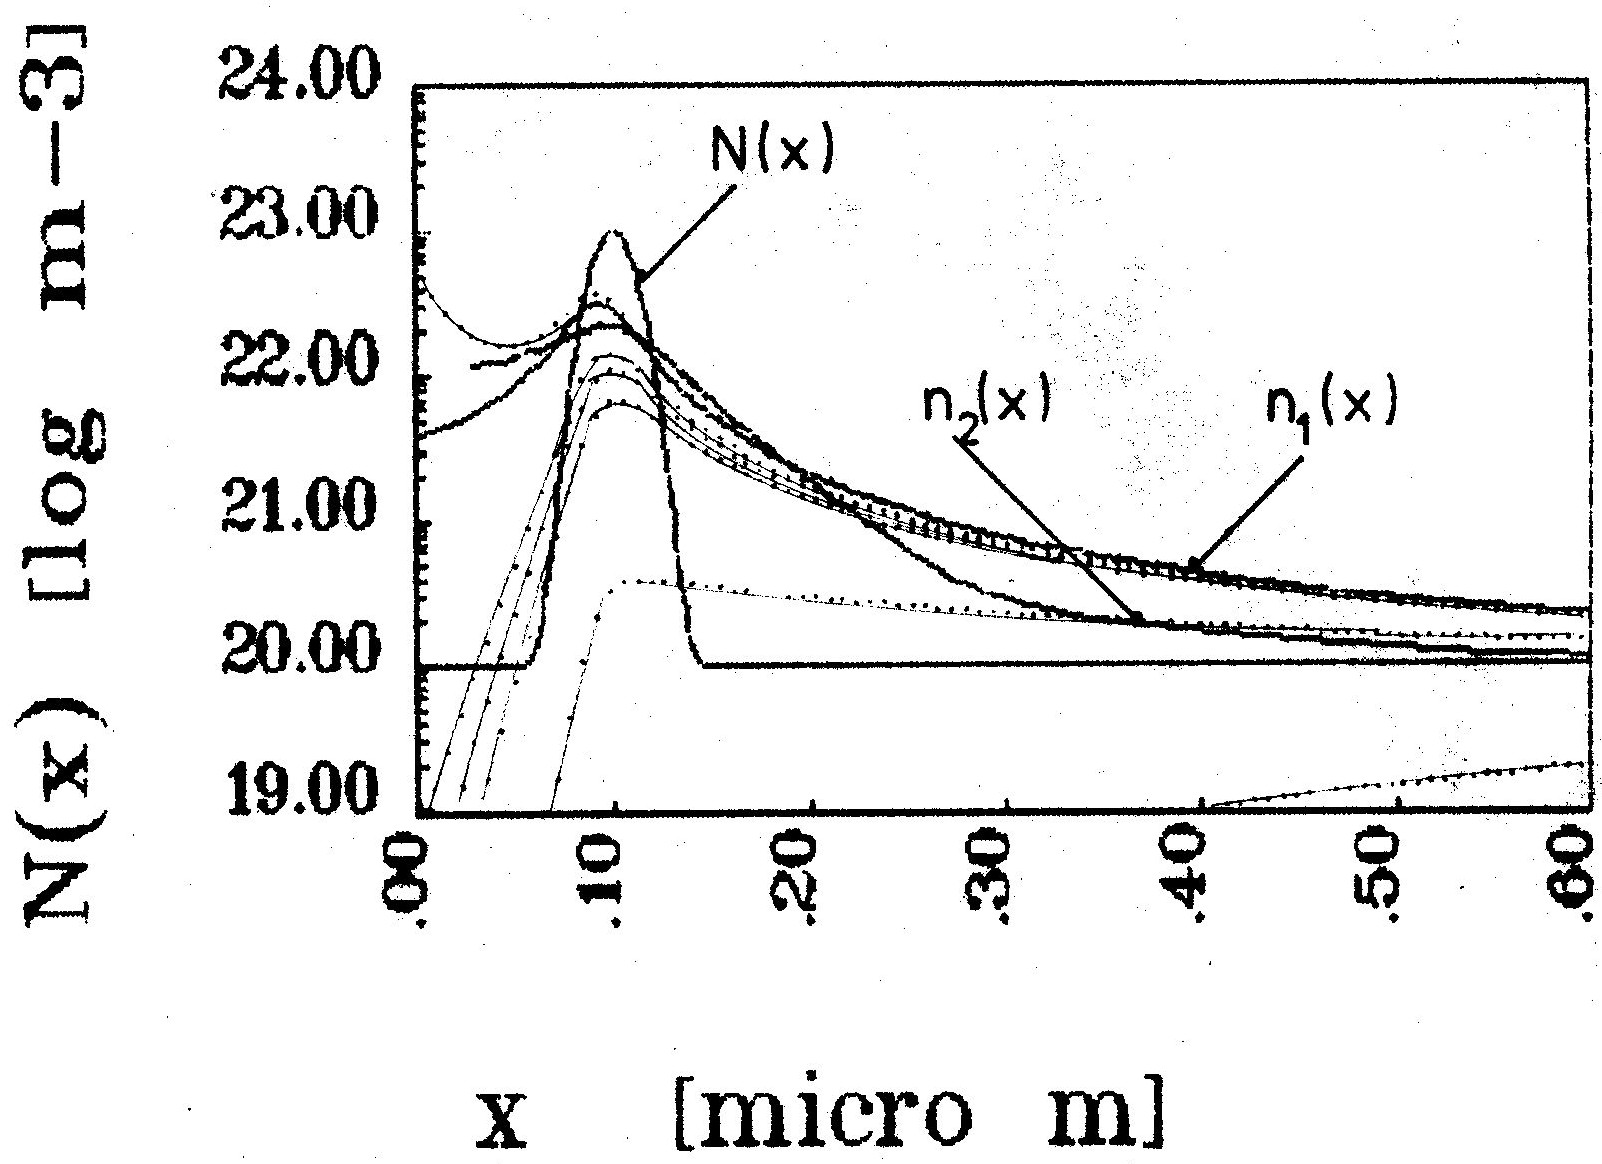
\includegraphics{Figures/fig-4-5.eps}
      \caption[Priebeh koncentrácie prímesí simulovaný Gaussovským
        rozložením]{Priebeh koncentrácie prímesí $N(x)$ simulovaný
        Gaussovským rozložením s parametrami $R_{p}=0.1\mu m$, $\Delta
        R_{p}=0.01\mu m$, $N_{\max}=1.0\times10^{23}m^{-3}$,
        $N_{bulk}=1.0\times10^{21}m^{-3}$; priebeh majoritných nosičov
        náboja $n_{1}(x)$ a priebeh $n_{2}(x)$, získaný z teoretickej
        C-V závislosti. Bodkovanými čiarami je znázornené
        ochudobňovanie štruktúry MOS.}\label{fig:4.5}
    \end{center}
  \end{minipage}
\end{figure}
%OBR25.BIT

\par Ďalšia analýza aproximácií, použitých pri výpočte koncentračných
profilov, by sa mohla zamerať na hľadanie exaktného obmedzenia
platnosti týchto aproximácií, avšak zo systematického hľadiska by bolo
pre riešenie tejto problematiky efektívnejšie zvoliť prístup, ku
ktorému sa vzťahuje nasledovná poznámka.

\begin{minipage}[c]{\textwidth}
  \emph{POZNÁMKA.} Pomocou kapacitných meraní by bolo možné určiť
  priebeh $N(x)$ presne bez použitia aproximácií uvedených v
  predchádzajúcich článkoch.  V práci~\cite{4.4} dodatku A je
  naznačený postup výpočtu elektrického potenciálu v polovodiči, ktorý
  je funkciou vzdialenosti (od povrchu polovodiča do hĺbky) a napätia
  hradla.  Deriváciou Poissonovej rovnice~\ref{eq:1.2} podľa $V_{g}$
  dostávame parciálnu diferenciálnu rovnicu tretieho rádu, ktorá
  presne opisuje experiment merania C-V závislosti
  \begin{equation}\label{eq:4.13}
    \frac{\delta^{3}\varphi}{\delta x^{2}\delta V_{g}} = {\frac{1}{L_{D}^{2}}}\ {e^{\beta\varphi}}\ {\frac{\delta\varphi}{\delta V_{g}}}
  \end{equation}
  Jej riešením použitím vhodných okrajových podmienok by bolo možné
  získať plochu $\varphi(x,V_{g})$, z ktorej pre výpočet $N(x)$ je
  potrebná len jedna priamka $\varphi(x)\rvert_{V_{g}}$
  \begin{equation}\label{eq:4.14}
    N(x) = N_{bulk}\ e^{\beta\varphi}-\frac{\epsilon}{q}\frac{\delta^{2}\varphi}{\delta x^{2}}
  \end{equation}
  (todo: check equation 4.14 in ref 4.4)
  Autori článku~\cite{4.4} túto metódu ďalej nerozvíjali z dôvodov
  ťažkosti pri vyčísľovaní druhej derivácie vo vzorci~\ref{eq:4.14}.
\end{minipage}

\section{Určenie hustoty pascí rozhrania $Si-SiO_{2}$.}\label{sec:4.2}

Kvalitu rozhrania $Si-SiO_{2}$ charakterizujeme hustotou pascí
rozhrania $(D_{it})$, ktorá je dôsledkom mechanizmu termickej oxidácie
kremíka, pri ktorej dochádza k vytvoreniu oblasti s nestechiometrickým
zložením. Túto hustotu možno vyhodnotiť následujúcimi dvoma postupmi:

\begin{enumerate}
\item Porovnanie nameranej vysokofrekvenčnej C-V závislosti
  $C_{mos}^{HF}(V_{g})$ a nameranej nízkofrekvenčnej C-V závislosti
  $C_{mos}^{LF}(V_{g})$. Vyhodnotenie $D_{it}$ pomocou porovnania
  uvedených závislostí vychádza z predpokladu, že závislosť
  $C_{mos}^{HF}(V_{g})$ je meraná dostatočne vysokým VF signálom, čo
  spôsobí, že kapacita nie je ovplyvnená pascami rozhrania
  $Si-SiO_{2}$.
\item Porovnanie nameranej závislosti $C_{mos}^{LF}(V_{g})$ a
  teoretickej nízkofrekvenčnej C-V závislosti, ktorú označíme
  $C_{mos}^{TLF}(V_{g})$.  V tomto prípade je potrebné na základe
  známeho priebehu koncentračného profilu dotujúcich prímesí v
  podpovrchovej oblasti polovodiča vypočítať závislosť
  $C_{mos}^{TLF}(V_{g})$ riešením Poissonovej rovnice.
\end{enumerate}

Pre vyhodnotenie $D_{it}$ sme použili obe metódy, ktorých realizáciu v
ďalšom podrobne uvedieme.

\subsection{Porovnanie vysokofrekvenčnej a nízkofrekvenčnej C-V závislosti.}\label{sec:4.2.1}

V tomto prípade využijeme frekvenčnú závislosť kapacity štruktúry MOS
a $D_{it}$ určíme z porovnania $C_{mos}^{HF}(V_{g})$ a
$C_{mos}^{LF}(V_{g})$. Potrebný teoretický základ možno nájsť
napríklad v~\cite{I.1}.  Pre určenie $C_{mos}^{HF}(V_{g})$ a
$C_{mos}^{LF}(V_{g})$ je vhodné použiť Q-C metódu~\cite{3.4, 3.6, 3.7,
  3.8}, ktorá umožňuje simultánne určenie oboch závislostí, avšak
použitie štandardných metód určovania $C_{mos}^{HF}(V_{g})$ a
$C_{mos}^{LF}(V_{g})$ je tiež možné.

Na obrázku~\ref{fig:4.6} sú namerané hodnoty $C_{mos}^{HF}(V_{g})$ a
povrchového potenciálu $\varphi_{s}$ štruktúry MOS, určené pomocou Q-C
metódy. Na obrázku~\ref{fig:4.7} sa nachádzajú krivky
$C_{mos}^{HF}(V_{g})$ a $C_{mos}^{LF}(V_{g})$, ktoré použijeme pre
výpočet $D_{it}$ podľa následujúceho vzťahu~\cite{4.15}

\begin{equation}\label{eq:4.15}
  D_{it} = {\cfrac{1}{q}} {\left[\cfrac{C_{mos}^{LF}}{1-\cfrac{C_{mos}^{LF}}{C_{ox}}} - \cfrac{C_{mos}^{HF}}{1-\cfrac{C_{mos}^{HF}}{C_{ox}}}\right]}
\end{equation}
% was (4.14) in origin

Polohu Fermiho hladiny v zakázanom pásme pre vypočítané hodnoty
$D_{it}$ určíme pomocou hodnôt povrchového potenciálu $\varphi_{s}$ a
vzdialenosti Fermiho hladiny od intrinzickej Fermiho hladiny
$\varphi_{f}$. Priebeh povrchového potenciálu $\varphi_{s}(V_{g})$
získame buď priamo pomocou Q-C metódy, alebo integráciou
kvázistatickej C-V závislosti použitím Berglundovho integrálu. V oboch
prípadoch dostávame priebehy $\varphi_{s}(V_{g})$, ktoré sú posunuté v
smere osi $y$. V prípade Q-C metódy sa jedná o konštantu
$\varphi_{s0}$, ktorá predstavuje povrchový potenciál, ak na hradle
štruktúry MOS nie je pripojené napätie a v prípade kvázistatickej C-V
metódy posunutie predstavuje integračnú konštantu. Pre obidva prípady
môžeme posunutie závislosti $\varphi_{s}(V_{g})$ vypočítať postupom
uvedeným v dodatku~\ref{app:AppendixG}.

\newpage
\begin{figure}[h!]\centering
  \begin{minipage}[c]{\myfiguresize}
    \begin{center}
      % GNUPLOT: LaTeX picture with Postscript
\begingroup
  \makeatletter
  \providecommand\color[2][]{%
    \GenericError{(gnuplot) \space\space\space\@spaces}{%
      Package color not loaded in conjunction with
      terminal option `colourtext'%
    }{See the gnuplot documentation for explanation.%
    }{Either use 'blacktext' in gnuplot or load the package
      color.sty in LaTeX.}%
    \renewcommand\color[2][]{}%
  }%
  \providecommand\includegraphics[2][]{%
    \GenericError{(gnuplot) \space\space\space\@spaces}{%
      Package graphicx or graphics not loaded%
    }{See the gnuplot documentation for explanation.%
    }{The gnuplot epslatex terminal needs graphicx.sty or graphics.sty.}%
    \renewcommand\includegraphics[2][]{}%
  }%
  \providecommand\rotatebox[2]{#2}%
  \@ifundefined{ifGPcolor}{%
    \newif\ifGPcolor
    \GPcolortrue
  }{}%
  \@ifundefined{ifGPblacktext}{%
    \newif\ifGPblacktext
    \GPblacktexttrue
  }{}%
  % define a \g@addto@macro without @ in the name:
  \let\gplgaddtomacro\g@addto@macro
  % define empty templates for all commands taking text:
  \gdef\gplbacktext{}%
  \gdef\gplfronttext{}%
  \makeatother
  \ifGPblacktext
    % no textcolor at all
    \def\colorrgb#1{}%
    \def\colorgray#1{}%
  \else
    % gray or color?
    \ifGPcolor
      \def\colorrgb#1{\color[rgb]{#1}}%
      \def\colorgray#1{\color[gray]{#1}}%
      \expandafter\def\csname LTw\endcsname{\color{white}}%
      \expandafter\def\csname LTb\endcsname{\color{black}}%
      \expandafter\def\csname LTa\endcsname{\color{black}}%
      \expandafter\def\csname LT0\endcsname{\color[rgb]{1,0,0}}%
      \expandafter\def\csname LT1\endcsname{\color[rgb]{0,1,0}}%
      \expandafter\def\csname LT2\endcsname{\color[rgb]{0,0,1}}%
      \expandafter\def\csname LT3\endcsname{\color[rgb]{1,0,1}}%
      \expandafter\def\csname LT4\endcsname{\color[rgb]{0,1,1}}%
      \expandafter\def\csname LT5\endcsname{\color[rgb]{1,1,0}}%
      \expandafter\def\csname LT6\endcsname{\color[rgb]{0,0,0}}%
      \expandafter\def\csname LT7\endcsname{\color[rgb]{1,0.3,0}}%
      \expandafter\def\csname LT8\endcsname{\color[rgb]{0.5,0.5,0.5}}%
    \else
      % gray
      \def\colorrgb#1{\color{black}}%
      \def\colorgray#1{\color[gray]{#1}}%
      \expandafter\def\csname LTw\endcsname{\color{white}}%
      \expandafter\def\csname LTb\endcsname{\color{black}}%
      \expandafter\def\csname LTa\endcsname{\color{black}}%
      \expandafter\def\csname LT0\endcsname{\color{black}}%
      \expandafter\def\csname LT1\endcsname{\color{black}}%
      \expandafter\def\csname LT2\endcsname{\color{black}}%
      \expandafter\def\csname LT3\endcsname{\color{black}}%
      \expandafter\def\csname LT4\endcsname{\color{black}}%
      \expandafter\def\csname LT5\endcsname{\color{black}}%
      \expandafter\def\csname LT6\endcsname{\color{black}}%
      \expandafter\def\csname LT7\endcsname{\color{black}}%
      \expandafter\def\csname LT8\endcsname{\color{black}}%
    \fi
  \fi
    \setlength{\unitlength}{0.0500bp}%
    \ifx\gptboxheight\undefined%
      \newlength{\gptboxheight}%
      \newlength{\gptboxwidth}%
      \newsavebox{\gptboxtext}%
    \fi%
    \setlength{\fboxrule}{0.5pt}%
    \setlength{\fboxsep}{1pt}%
\begin{picture}(7920.00,5182.00)%
    \gplgaddtomacro\gplbacktext{%
      \csname LTb\endcsname%%
      \put(740,640){\makebox(0,0)[r]{\strut{}$0.5$}}%
      \put(740,1203){\makebox(0,0)[r]{\strut{}$0.6$}}%
      \put(740,1766){\makebox(0,0)[r]{\strut{}$0.7$}}%
      \put(740,2329){\makebox(0,0)[r]{\strut{}$0.8$}}%
      \put(740,2892){\makebox(0,0)[r]{\strut{}$0.9$}}%
      \put(740,3455){\makebox(0,0)[r]{\strut{}$1$}}%
      \put(740,4018){\makebox(0,0)[r]{\strut{}$1.1$}}%
      \put(740,4581){\makebox(0,0)[r]{\strut{}$1.2$}}%
      \put(860,440){\makebox(0,0){\strut{}$-2$}}%
      \put(1697,440){\makebox(0,0){\strut{}$-1$}}%
      \put(2535,440){\makebox(0,0){\strut{}$0$}}%
      \put(3372,440){\makebox(0,0){\strut{}$1$}}%
      \put(4210,440){\makebox(0,0){\strut{}$2$}}%
      \put(5047,440){\makebox(0,0){\strut{}$3$}}%
      \put(5884,440){\makebox(0,0){\strut{}$4$}}%
      \put(6722,440){\makebox(0,0){\strut{}$5$}}%
      \put(7559,440){\makebox(0,0){\strut{}$6$}}%
    }%
    \gplgaddtomacro\gplfronttext{%
      \csname LTb\endcsname%%
      \put(190,2610){\rotatebox{-270}{\makebox(0,0){\strut{}${C}/{C}_{ox}$ \qquad $(1-{\varphi}/{\varphi}_{norm})$}}}%
      \put(4209,140){\makebox(0,0){\strut{}Napätie hradla ${V}_g$}}%
      \put(4209,4881){\makebox(0,0){\strut{}QC metóda}}%
      \csname LTb\endcsname%%
      \put(6142,1514){\makebox(0,0)[l]{\strut{}${C}_{mos}^{HF}$}}%
      \csname LTb\endcsname%%
      \put(6142,2293){\makebox(0,0)[l]{\strut{}${\varphi}_{s}^{HF}$}}%
    }%
    \gplbacktext
    \put(0,0){\includegraphics{/export/scratch/vbotka-thesis/Plot/Figures/fig-4-6-sk}}%
    \gplfronttext
  \end{picture}%
\endgroup

      \caption[VF C-V závislosť $C_{mos}^{HF}(V_{g})$ a priebeh
        povrchového potenciálu $\varphi_{s}(V_{g})$ štruktúry MOS
        získané pomocou Q-C metódy]{VF C-V závislosť
        $C_{mos}^{HF}(V_{g})$ normovaná na $C_{ox}$ a normovaný
        povrchový potenciál $\varphi_{s}(V_{g})$ získaný pomocou Q-C
        metódy. Povrchový potenciál je normovaný vzťahom
        $1-{\varphi_{s}}/{\varphi_{norm}}$, kde
        $\varphi_{norm}=3.33$.}\label{fig:4.6}
    \end{center}
  \end{minipage}
\end{figure}
% OBR15.BIT

\begin{figure}[h!]\centering
  \begin{minipage}[c]{\myfiguresize}
    \begin{center}
      % GNUPLOT: LaTeX picture with Postscript
\begingroup
  \makeatletter
  \providecommand\color[2][]{%
    \GenericError{(gnuplot) \space\space\space\@spaces}{%
      Package color not loaded in conjunction with
      terminal option `colourtext'%
    }{See the gnuplot documentation for explanation.%
    }{Either use 'blacktext' in gnuplot or load the package
      color.sty in LaTeX.}%
    \renewcommand\color[2][]{}%
  }%
  \providecommand\includegraphics[2][]{%
    \GenericError{(gnuplot) \space\space\space\@spaces}{%
      Package graphicx or graphics not loaded%
    }{See the gnuplot documentation for explanation.%
    }{The gnuplot epslatex terminal needs graphicx.sty or graphics.sty.}%
    \renewcommand\includegraphics[2][]{}%
  }%
  \providecommand\rotatebox[2]{#2}%
  \@ifundefined{ifGPcolor}{%
    \newif\ifGPcolor
    \GPcolortrue
  }{}%
  \@ifundefined{ifGPblacktext}{%
    \newif\ifGPblacktext
    \GPblacktexttrue
  }{}%
  % define a \g@addto@macro without @ in the name:
  \let\gplgaddtomacro\g@addto@macro
  % define empty templates for all commands taking text:
  \gdef\gplbacktext{}%
  \gdef\gplfronttext{}%
  \makeatother
  \ifGPblacktext
    % no textcolor at all
    \def\colorrgb#1{}%
    \def\colorgray#1{}%
  \else
    % gray or color?
    \ifGPcolor
      \def\colorrgb#1{\color[rgb]{#1}}%
      \def\colorgray#1{\color[gray]{#1}}%
      \expandafter\def\csname LTw\endcsname{\color{white}}%
      \expandafter\def\csname LTb\endcsname{\color{black}}%
      \expandafter\def\csname LTa\endcsname{\color{black}}%
      \expandafter\def\csname LT0\endcsname{\color[rgb]{1,0,0}}%
      \expandafter\def\csname LT1\endcsname{\color[rgb]{0,1,0}}%
      \expandafter\def\csname LT2\endcsname{\color[rgb]{0,0,1}}%
      \expandafter\def\csname LT3\endcsname{\color[rgb]{1,0,1}}%
      \expandafter\def\csname LT4\endcsname{\color[rgb]{0,1,1}}%
      \expandafter\def\csname LT5\endcsname{\color[rgb]{1,1,0}}%
      \expandafter\def\csname LT6\endcsname{\color[rgb]{0,0,0}}%
      \expandafter\def\csname LT7\endcsname{\color[rgb]{1,0.3,0}}%
      \expandafter\def\csname LT8\endcsname{\color[rgb]{0.5,0.5,0.5}}%
    \else
      % gray
      \def\colorrgb#1{\color{black}}%
      \def\colorgray#1{\color[gray]{#1}}%
      \expandafter\def\csname LTw\endcsname{\color{white}}%
      \expandafter\def\csname LTb\endcsname{\color{black}}%
      \expandafter\def\csname LTa\endcsname{\color{black}}%
      \expandafter\def\csname LT0\endcsname{\color{black}}%
      \expandafter\def\csname LT1\endcsname{\color{black}}%
      \expandafter\def\csname LT2\endcsname{\color{black}}%
      \expandafter\def\csname LT3\endcsname{\color{black}}%
      \expandafter\def\csname LT4\endcsname{\color{black}}%
      \expandafter\def\csname LT5\endcsname{\color{black}}%
      \expandafter\def\csname LT6\endcsname{\color{black}}%
      \expandafter\def\csname LT7\endcsname{\color{black}}%
      \expandafter\def\csname LT8\endcsname{\color{black}}%
    \fi
  \fi
    \setlength{\unitlength}{0.0500bp}%
    \ifx\gptboxheight\undefined%
      \newlength{\gptboxheight}%
      \newlength{\gptboxwidth}%
      \newsavebox{\gptboxtext}%
    \fi%
    \setlength{\fboxrule}{0.5pt}%
    \setlength{\fboxsep}{1pt}%
\begin{picture}(7920.00,5616.00)%
    \gplgaddtomacro\gplbacktext{%
      \csname LTb\endcsname%%
      \put(740,640){\makebox(0,0)[r]{\strut{}$0.5$}}%
      \put(740,1265){\makebox(0,0)[r]{\strut{}$0.6$}}%
      \put(740,1890){\makebox(0,0)[r]{\strut{}$0.7$}}%
      \put(740,2515){\makebox(0,0)[r]{\strut{}$0.8$}}%
      \put(740,3140){\makebox(0,0)[r]{\strut{}$0.9$}}%
      \put(740,3765){\makebox(0,0)[r]{\strut{}$1$}}%
      \put(740,4390){\makebox(0,0)[r]{\strut{}$1.1$}}%
      \put(740,5015){\makebox(0,0)[r]{\strut{}$1.2$}}%
      \put(860,440){\makebox(0,0){\strut{}$-2$}}%
      \put(1697,440){\makebox(0,0){\strut{}$-1$}}%
      \put(2535,440){\makebox(0,0){\strut{}$0$}}%
      \put(3372,440){\makebox(0,0){\strut{}$1$}}%
      \put(4210,440){\makebox(0,0){\strut{}$2$}}%
      \put(5047,440){\makebox(0,0){\strut{}$3$}}%
      \put(5884,440){\makebox(0,0){\strut{}$4$}}%
      \put(6722,440){\makebox(0,0){\strut{}$5$}}%
      \put(7559,440){\makebox(0,0){\strut{}$6$}}%
    }%
    \gplgaddtomacro\gplfronttext{%
      \csname LTb\endcsname%%
      \put(190,2827){\rotatebox{-270}{\makebox(0,0){\strut{}${C}/{C}_{ox}$}}}%
      \put(4209,140){\makebox(0,0){\strut{}Napätie hradla ${V}_g$}}%
      \put(4209,5315){\makebox(0,0){\strut{}QC metóda}}%
      \csname LTb\endcsname%%
      \put(5733,1615){\makebox(0,0)[l]{\strut{}${C}_{mos}^{HF}$}}%
      \csname LTb\endcsname%%
      \put(5733,3621){\makebox(0,0)[l]{\strut{}${C}_{mos}^{LF}$}}%
    }%
    \gplbacktext
    \put(0,0){\includegraphics{/export/scratch/vbotka-thesis/Plot/Figures/fig-4-7-sk}}%
    \gplfronttext
  \end{picture}%
\endgroup

      \caption[VF C-V závislosť $C_{mos}^{HF}(V_{g})$ a LF C-V
        závislosť $C_{mos}^{LF}(V_{g})$ štruktúry MOS normované na
        kapacitu oxidu, získané pomocou Q-C metódy]{VF C-V závislosť
        $C_{mos}^{HF}(V_{g})$ a LF C-V závislosť $C_{mos}^{LF}(V_{g})$
        štruktúry MOS normované na kapacitu oxidu, získané pomocou Q-C
        metódy.  LF C-V závislosť je vypočítaná deriváciou povrchového
        potenciálu (zobrazeného na obrázku~\ref{fig:4.6}) podľa
        vzťahu~\ref{eq:3.2}.}\label{fig:4.7}
    \end{center}
  \end{minipage}
\end{figure}
% OBR12.BIT

\newpage
\begin{figure}[h!]\centering
  \begin{minipage}[c]{\myfiguresize}
    \begin{center}
      % GNUPLOT: LaTeX picture with Postscript
\begingroup
  \makeatletter
  \providecommand\color[2][]{%
    \GenericError{(gnuplot) \space\space\space\@spaces}{%
      Package color not loaded in conjunction with
      terminal option `colourtext'%
    }{See the gnuplot documentation for explanation.%
    }{Either use 'blacktext' in gnuplot or load the package
      color.sty in LaTeX.}%
    \renewcommand\color[2][]{}%
  }%
  \providecommand\includegraphics[2][]{%
    \GenericError{(gnuplot) \space\space\space\@spaces}{%
      Package graphicx or graphics not loaded%
    }{See the gnuplot documentation for explanation.%
    }{The gnuplot epslatex terminal needs graphicx.sty or graphics.sty.}%
    \renewcommand\includegraphics[2][]{}%
  }%
  \providecommand\rotatebox[2]{#2}%
  \@ifundefined{ifGPcolor}{%
    \newif\ifGPcolor
    \GPcolortrue
  }{}%
  \@ifundefined{ifGPblacktext}{%
    \newif\ifGPblacktext
    \GPblacktexttrue
  }{}%
  % define a \g@addto@macro without @ in the name:
  \let\gplgaddtomacro\g@addto@macro
  % define empty templates for all commands taking text:
  \gdef\gplbacktext{}%
  \gdef\gplfronttext{}%
  \makeatother
  \ifGPblacktext
    % no textcolor at all
    \def\colorrgb#1{}%
    \def\colorgray#1{}%
  \else
    % gray or color?
    \ifGPcolor
      \def\colorrgb#1{\color[rgb]{#1}}%
      \def\colorgray#1{\color[gray]{#1}}%
      \expandafter\def\csname LTw\endcsname{\color{white}}%
      \expandafter\def\csname LTb\endcsname{\color{black}}%
      \expandafter\def\csname LTa\endcsname{\color{black}}%
      \expandafter\def\csname LT0\endcsname{\color[rgb]{1,0,0}}%
      \expandafter\def\csname LT1\endcsname{\color[rgb]{0,1,0}}%
      \expandafter\def\csname LT2\endcsname{\color[rgb]{0,0,1}}%
      \expandafter\def\csname LT3\endcsname{\color[rgb]{1,0,1}}%
      \expandafter\def\csname LT4\endcsname{\color[rgb]{0,1,1}}%
      \expandafter\def\csname LT5\endcsname{\color[rgb]{1,1,0}}%
      \expandafter\def\csname LT6\endcsname{\color[rgb]{0,0,0}}%
      \expandafter\def\csname LT7\endcsname{\color[rgb]{1,0.3,0}}%
      \expandafter\def\csname LT8\endcsname{\color[rgb]{0.5,0.5,0.5}}%
    \else
      % gray
      \def\colorrgb#1{\color{black}}%
      \def\colorgray#1{\color[gray]{#1}}%
      \expandafter\def\csname LTw\endcsname{\color{white}}%
      \expandafter\def\csname LTb\endcsname{\color{black}}%
      \expandafter\def\csname LTa\endcsname{\color{black}}%
      \expandafter\def\csname LT0\endcsname{\color{black}}%
      \expandafter\def\csname LT1\endcsname{\color{black}}%
      \expandafter\def\csname LT2\endcsname{\color{black}}%
      \expandafter\def\csname LT3\endcsname{\color{black}}%
      \expandafter\def\csname LT4\endcsname{\color{black}}%
      \expandafter\def\csname LT5\endcsname{\color{black}}%
      \expandafter\def\csname LT6\endcsname{\color{black}}%
      \expandafter\def\csname LT7\endcsname{\color{black}}%
      \expandafter\def\csname LT8\endcsname{\color{black}}%
    \fi
  \fi
    \setlength{\unitlength}{0.0500bp}%
    \ifx\gptboxheight\undefined%
      \newlength{\gptboxheight}%
      \newlength{\gptboxwidth}%
      \newsavebox{\gptboxtext}%
    \fi%
    \setlength{\fboxrule}{0.5pt}%
    \setlength{\fboxsep}{1pt}%
\begin{picture}(7920.00,5616.00)%
    \gplgaddtomacro\gplbacktext{%
      \csname LTb\endcsname%%
      \put(1100,640){\makebox(0,0)[r]{\strut{}$1\times10^{7}$}}%
      \put(1100,2098){\makebox(0,0)[r]{\strut{}$1\times10^{8}$}}%
      \put(1100,3557){\makebox(0,0)[r]{\strut{}$1\times10^{9}$}}%
      \put(1100,5015){\makebox(0,0)[r]{\strut{}$1\times10^{10}$}}%
      \put(1220,440){\makebox(0,0){\strut{}$0$}}%
      \put(2012,440){\makebox(0,0){\strut{}$0.05$}}%
      \put(2805,440){\makebox(0,0){\strut{}$0.1$}}%
      \put(3597,440){\makebox(0,0){\strut{}$0.15$}}%
      \put(4390,440){\makebox(0,0){\strut{}$0.2$}}%
      \put(5182,440){\makebox(0,0){\strut{}$0.25$}}%
      \put(5974,440){\makebox(0,0){\strut{}$0.3$}}%
      \put(6767,440){\makebox(0,0){\strut{}$0.35$}}%
      \put(7559,440){\makebox(0,0){\strut{}$0.4$}}%
    }%
    \gplgaddtomacro\gplfronttext{%
      \csname LTb\endcsname%%
      \put(190,2827){\rotatebox{-270}{\makebox(0,0){\strut{}$D_{it} [m^{-2}eV^{-1}]$}}}%
      \put(4389,140){\makebox(0,0){\strut{}$E_{c} - E [eV]$}}%
      \put(4389,5315){\makebox(0,0){\strut{}Hustota pascí rozhrania $Si-SiO_{2}$}}%
    }%
    \gplbacktext
    \put(0,0){\includegraphics{/export/scratch/vbotka-thesis/Plot/Figures/fig-4-8-sk}}%
    \gplfronttext
  \end{picture}%
\endgroup

      \caption[Závislosť $D_{it}$ od polohy v zakázanom pásme
        polovodiča typu P, určená z porovnania $C_{mos}^{HF}(V_{g})$ a
        $C_{mos}^{LF}(V_{g})$]{Závislosť $D_{it}$ od polohy v
        zakázanom pásme polovodiča typu P, určená z porovnania
        $C_{mos}^{HF}(V_{g})$ a $C_{mos}^{LF}(V_{g})$, ktoré sú
        zobrazené na obrázku~\ref{fig:4.7}.}\label{fig:4.8}
    \end{center}
  \end{minipage}
\end{figure}
% OBR14.BIT

Hodnotu potenciálu $\varphi_{f}$ určíme pomocou vzťahu

\begin{equation}\label{eq:4.16}
  \varphi_{f} = \pm \frac{kT}{g} \ln{\frac{N_{b}}{n_{i}}}
\end{equation}

, kde predpokladáme znalosť koncentrácie substrátu $N_{b}$. Potenciál
$\varphi_{f}$ má kladné znamienko pre polovodič typu P. Ak pre
povrchový potenciál $\varphi_{s}$ zvolíme tú istú orientáciu ako pre
potenciál $\varphi_{f}$, energetickú polohu pascí rozhrania v
zakázanom pásme potom určíme pomocou nasledovného vzťahu

\begin{equation}\label{eq:4.17}
  E_{c} - E = 0.56 + \varphi_{s} + \varphi_{f}
\end{equation}

,kde číslo $0.56$ predstavuje vzdialenosť dolného okraja vodivostného
pásma $(E_{c})$ od intrinzickej Fermiho hladiny. Priebeh $D_{it}$ ako
funkcie polohy v zakázanom pásme je znázornený na
obrázku~\ref{fig:4.8}.

\newpage
\subsection{Porovnanie experimentálnej a teoretickej kvázistatickej CV závislosti.}\label{sec:4.2.2}

Pre výpočet $D_{it}$ pomocou tejto metódy je potrebné poznať priebeh
koncentračného profilu dotujúcich prímesí v podpovrchovej oblasti
polovodiča $N(x)$, aby sme mohli vypočítať
$C_{mos}^{TLF}(V_{g})$. Teoretickú závislosť $C_{mos}^{TLF}(V_{g})$
štruktúry MOS vypočítame numerickým postupom popísaným v
dodatku~\ref{app:AppendixA}.  Použitie numerických metód je v tomto
prípade nevyhnutné, pretože analytické riešenie Poissonovej rovnice
nie je možné pre všeobecný priebeh koncentrácie $N(x)$.  Pri
numerickom riešení Poissonovej rovnice zároveň vypočítame závislosť
povrchového potenciálu od napätia hradla $\varphi_{s}(V_{g})$, ktorú
použijeme pre určenie pozície vypočítanej hustoty pascí rozhrania v
zakázanom pásme polovodiča.  Pretože počas numerického výpočtu
neberieme do úvahy poruchové náboje v oxidovej vrstve a na rozhraní
$Si-SiO_{2}$ obidve teoreticky určené závislosti $\varphi_{s}(V_{g})$
aj $C_{mos}^{TLF}(V_{g})$ budú posunuté voči nameranej kvázistatickej
C-V závislosti o hodnotu $V_{FB}$. Pre posunutie uvedených závislostí
musíme poznať aj hodnotu $V_{FB}$.

\par Pre výpočet $D_{it}$ teda použijeme $C_{mos}^{TLF}(V_{g})$, ktorá
nie je zaťažená kapacitou pascí rozhrania $Si-SiO_{2}$. Na
obrázku~\ref{fig:4.9} sú zobrazené nameraná a teoretická LF C-V
závislosť, ktoré ďalej použijeme na vyhodnotenie $D_{it}$ podľa
vzťahu

\begin{equation}\label{eq:4.18}
  D_{it} = {\cfrac{1}{q}} {\left[\cfrac{C_{mos}^{LF}}{1-\cfrac{C_{mos}^{LF}}{C_{ox}}}-\cfrac{C_{mos}^{TLF}}{1-\cfrac{C_{mos}^{TLF}}{C_{ox}}}\right]}
\end{equation}

Na obrázku~\ref{fig:4.10} je znázornený priebeh hustoty pascí
rozhrania v závislosti od polohy v zakázanom pásme polovodiča určený
uvedeným spôsobom.  Nevýhoda popísanej metódy spočíva v časovej
náročnosti výpočtu teoretickej nízkofrekvenčnej C-V
závislosti. Napriek tomu, že porovnanie teoretickej a experimentálnej
nízkofrekvenčnej C-V závislosti poskytuje hodnoty$D_{it}$ vo väčšej
oblasti zakázaného pásma, pre vyhodnocovanie plošného rozloženia
$D_{it}$ na kremíkovej doske sme z časových dôvodov použili postup
popísaný v časti~\ref{sec:4.2.1}

\begin{figure}[h!]\centering
  \begin{minipage}[c]{\myfiguresize}
    \begin{center}
      % GNUPLOT: LaTeX picture with Postscript
\begingroup
  \makeatletter
  \providecommand\color[2][]{%
    \GenericError{(gnuplot) \space\space\space\@spaces}{%
      Package color not loaded in conjunction with
      terminal option `colourtext'%
    }{See the gnuplot documentation for explanation.%
    }{Either use 'blacktext' in gnuplot or load the package
      color.sty in LaTeX.}%
    \renewcommand\color[2][]{}%
  }%
  \providecommand\includegraphics[2][]{%
    \GenericError{(gnuplot) \space\space\space\@spaces}{%
      Package graphicx or graphics not loaded%
    }{See the gnuplot documentation for explanation.%
    }{The gnuplot epslatex terminal needs graphicx.sty or graphics.sty.}%
    \renewcommand\includegraphics[2][]{}%
  }%
  \providecommand\rotatebox[2]{#2}%
  \@ifundefined{ifGPcolor}{%
    \newif\ifGPcolor
    \GPcolortrue
  }{}%
  \@ifundefined{ifGPblacktext}{%
    \newif\ifGPblacktext
    \GPblacktexttrue
  }{}%
  % define a \g@addto@macro without @ in the name:
  \let\gplgaddtomacro\g@addto@macro
  % define empty templates for all commands taking text:
  \gdef\gplbacktext{}%
  \gdef\gplfronttext{}%
  \makeatother
  \ifGPblacktext
    % no textcolor at all
    \def\colorrgb#1{}%
    \def\colorgray#1{}%
  \else
    % gray or color?
    \ifGPcolor
      \def\colorrgb#1{\color[rgb]{#1}}%
      \def\colorgray#1{\color[gray]{#1}}%
      \expandafter\def\csname LTw\endcsname{\color{white}}%
      \expandafter\def\csname LTb\endcsname{\color{black}}%
      \expandafter\def\csname LTa\endcsname{\color{black}}%
      \expandafter\def\csname LT0\endcsname{\color[rgb]{1,0,0}}%
      \expandafter\def\csname LT1\endcsname{\color[rgb]{0,1,0}}%
      \expandafter\def\csname LT2\endcsname{\color[rgb]{0,0,1}}%
      \expandafter\def\csname LT3\endcsname{\color[rgb]{1,0,1}}%
      \expandafter\def\csname LT4\endcsname{\color[rgb]{0,1,1}}%
      \expandafter\def\csname LT5\endcsname{\color[rgb]{1,1,0}}%
      \expandafter\def\csname LT6\endcsname{\color[rgb]{0,0,0}}%
      \expandafter\def\csname LT7\endcsname{\color[rgb]{1,0.3,0}}%
      \expandafter\def\csname LT8\endcsname{\color[rgb]{0.5,0.5,0.5}}%
    \else
      % gray
      \def\colorrgb#1{\color{black}}%
      \def\colorgray#1{\color[gray]{#1}}%
      \expandafter\def\csname LTw\endcsname{\color{white}}%
      \expandafter\def\csname LTb\endcsname{\color{black}}%
      \expandafter\def\csname LTa\endcsname{\color{black}}%
      \expandafter\def\csname LT0\endcsname{\color{black}}%
      \expandafter\def\csname LT1\endcsname{\color{black}}%
      \expandafter\def\csname LT2\endcsname{\color{black}}%
      \expandafter\def\csname LT3\endcsname{\color{black}}%
      \expandafter\def\csname LT4\endcsname{\color{black}}%
      \expandafter\def\csname LT5\endcsname{\color{black}}%
      \expandafter\def\csname LT6\endcsname{\color{black}}%
      \expandafter\def\csname LT7\endcsname{\color{black}}%
      \expandafter\def\csname LT8\endcsname{\color{black}}%
    \fi
  \fi
    \setlength{\unitlength}{0.0500bp}%
    \ifx\gptboxheight\undefined%
      \newlength{\gptboxheight}%
      \newlength{\gptboxwidth}%
      \newsavebox{\gptboxtext}%
    \fi%
    \setlength{\fboxrule}{0.5pt}%
    \setlength{\fboxsep}{1pt}%
\begin{picture}(7920.00,5616.00)%
    \gplgaddtomacro\gplbacktext{%
      \csname LTb\endcsname%%
      \put(740,640){\makebox(0,0)[r]{\strut{}$0.5$}}%
      \put(740,1265){\makebox(0,0)[r]{\strut{}$0.6$}}%
      \put(740,1890){\makebox(0,0)[r]{\strut{}$0.7$}}%
      \put(740,2515){\makebox(0,0)[r]{\strut{}$0.8$}}%
      \put(740,3140){\makebox(0,0)[r]{\strut{}$0.9$}}%
      \put(740,3765){\makebox(0,0)[r]{\strut{}$1$}}%
      \put(740,4390){\makebox(0,0)[r]{\strut{}$1.1$}}%
      \put(740,5015){\makebox(0,0)[r]{\strut{}$1.2$}}%
      \put(860,440){\makebox(0,0){\strut{}$-2$}}%
      \put(1977,440){\makebox(0,0){\strut{}$-1$}}%
      \put(3093,440){\makebox(0,0){\strut{}$0$}}%
      \put(4210,440){\makebox(0,0){\strut{}$1$}}%
      \put(5326,440){\makebox(0,0){\strut{}$2$}}%
      \put(6443,440){\makebox(0,0){\strut{}$3$}}%
      \put(7559,440){\makebox(0,0){\strut{}$4$}}%
    }%
    \gplgaddtomacro\gplfronttext{%
      \csname LTb\endcsname%%
      \put(190,2827){\rotatebox{-270}{\makebox(0,0){\strut{}${C}/{C}_{ox}$}}}%
      \put(4209,140){\makebox(0,0){\strut{}Napätie hradla ${V}_g$}}%
      \put(4209,5315){\makebox(0,0){\strut{}Porovnanie nameranej a reoretickej LF C-V}}%
      \csname LTb\endcsname%%
      \put(6780,3423){\makebox(0,0)[l]{\strut{}${C}_{mos}^{LF}$}}%
    }%
    \gplbacktext
    \put(0,0){\includegraphics{/export/scratch/vbotka-thesis/Plot/Figures/fig-4-9-sk}}%
    \gplfronttext
  \end{picture}%
\endgroup

      \caption[Teoretická LF C-V závislosť a nameraná LF C-V
        závislosť]{Teoretická LF C-V závislosť a nameraná LF C-V
        závislosť štruktúry MOS normované na kapacitu
        oxidu.}\label{fig:4.9}
    \end{center}
  \end{minipage}
\end{figure}
% OBR11.BIT

\begin{figure}[h!]\centering
  \begin{minipage}[c]{\myfiguresize}
    \begin{center}
      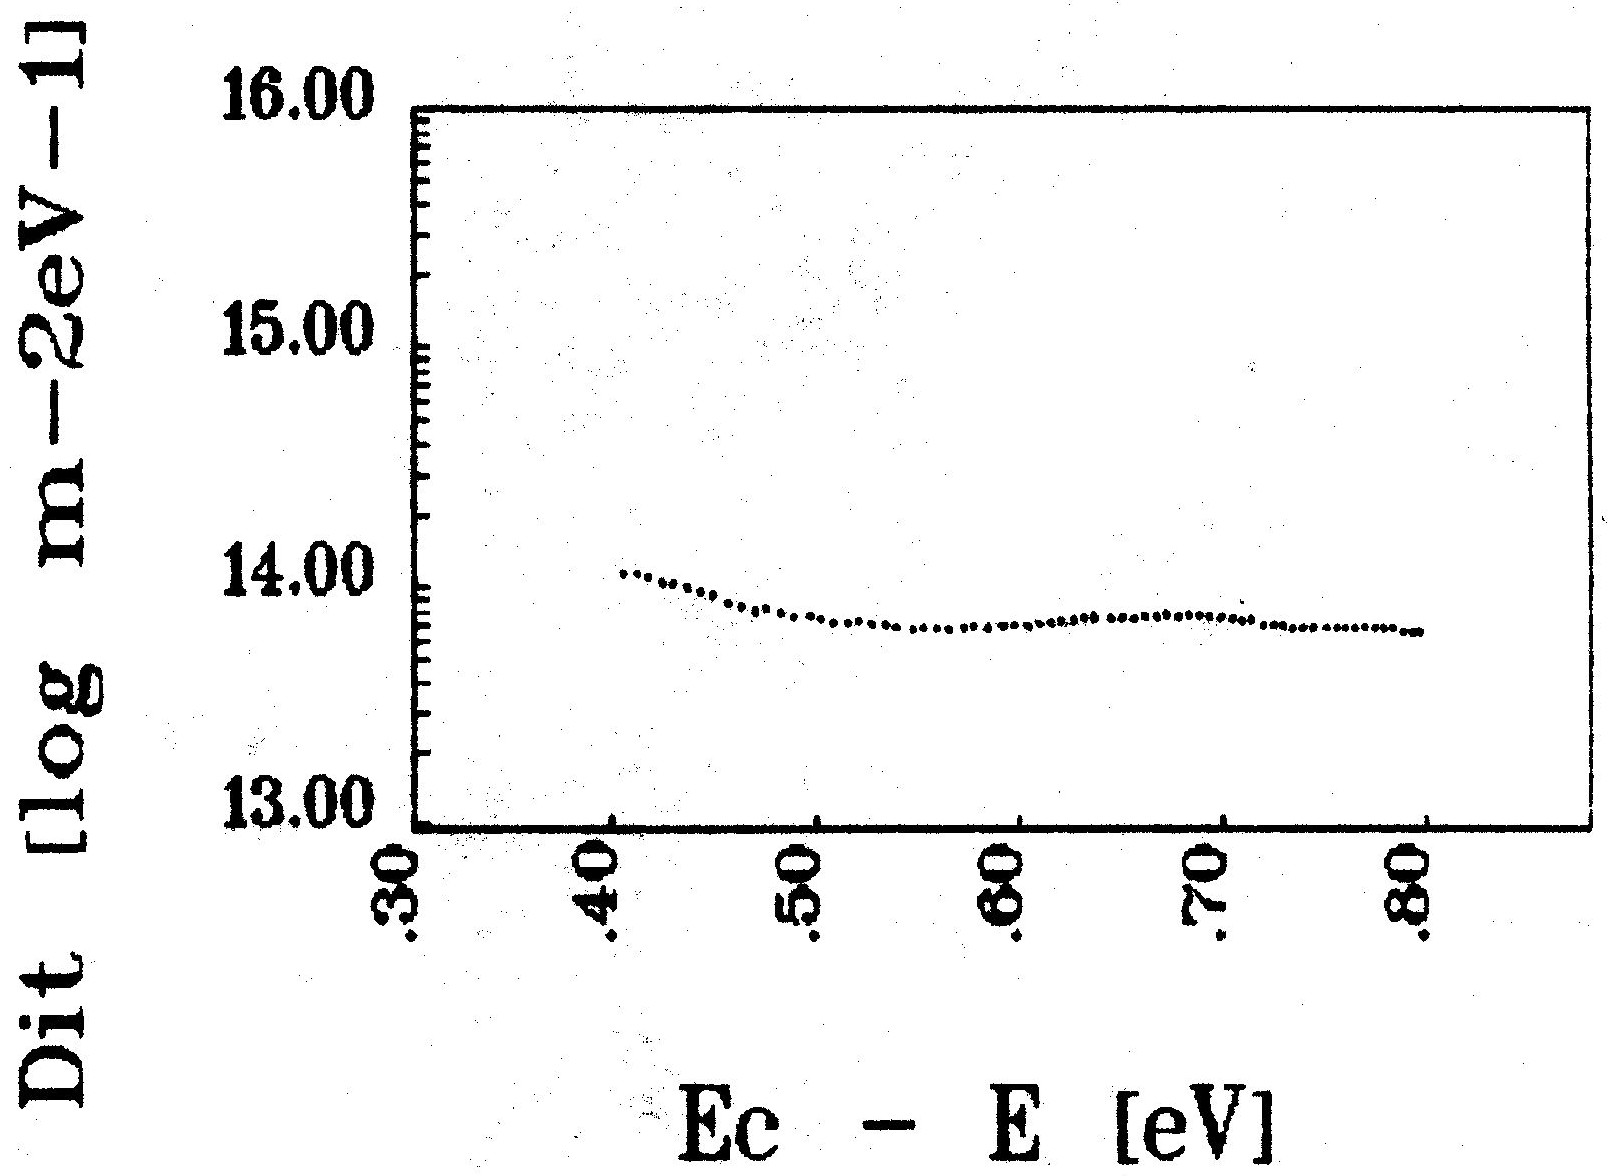
\includegraphics{Figures/fig-4-10.eps}
      \caption[Závislosť $D_{it}$ od polohy v zakázanom pásme
        polovodiča určená z porovnania $C_{mos}^{TLF}(V_{g})$ a
        $C_{mos}^{LF}(V_{g})$]{Závislosť $D_{it}$ od polohy v
        zakázanom pásme polovodiča typu P, určená z porovnania
        $C_{mos}^{TLF}(V_{g})$ a $C_{mos}^{LF}(V_{g})$, ktoré sú
        zobrazené na obrázku~\ref{fig:4.9}.}\label{fig:4.10}
    \end{center}
  \end{minipage}
\end{figure}
% OBR13.BIT


\begin{thebibliography}{}
\bibitem[4.1]{4.1} Lehovec K.: Solid St\.  Electron.  27 (1984)
  s.1907.
\bibitem[4.2]{4.2} Wu Chung P., Douglas E.C., Mueller C.W.: IEEE
  Trans.\ on elektron.\ dev. 22 (1975) s.319.
\bibitem[4.3]{4.3} Kroemer H., Chien W.: Solid St.\ Electron. 24
  (1981) s.655.
\bibitem[4.4]{4.4} Baccarani G., Rudan M., Maes H., Vandervorst W.,
  Van Overstraeten R.: Solid St\. Electron. 23 (1980) s. 65.
\bibitem[4.5]{4.5} Botka V., Csabay O., Artz P., Beyer A.: 3.vedecká
  konferencia EF SVŠT Elektrotechnika '90, EF SVŠT Bratislava, 1990
  s.73.
\bibitem[4.6]{4.6} Kinder R.: Príspevok ku skúmaniu koncentračných
  profilov implantovaných vrstiev. Kandidátska dizertačná práca. EF
  SVŠT Bratislava 1984.
\bibitem[4.7]{4.7} Lin S.T., Reuter J.: Solid St.\ Electron. 26 (1983)
  s.343.
\bibitem[4.8]{4.8} Ziegler K., Klausmann E.: Solid St.\ Electron. 18
  (1975) s.189.
\bibitem[4.9]{4.9} Jindal R.P., Warner R.M. Jr.: IEEE Trans.\ on
  elektron.\ dev. 28 (1981) s.348.
\bibitem[4.10]{4.10} Jindal R.P.: Solid St.\ Electron. 26 (1983)
  s.1005.
\bibitem[4.11]{4.11} Warner R.M. Jr., Jindal R.P.: Solid
  St.\ Electron. 26 (1983) s.335.
\bibitem[4.12]{4.12} Balland B., Remaki B., Marchand J.J.:
  J. Phys. E. Sci. Instrum. 21 (1988) s.559.
\bibitem[4.13]{4.13} Csabay O., Botka V.: 5.celoštátna konferencia
  Mikroelektronika 1989, Dom techniky ČSVTS Bratislava, 1989 s.58.
\bibitem[4.14]{4.14} Zsalkovics G.: Určovanie koncentračného profilu
  implantovanej vrstvy z kapacitných meraní. Diplomová práca, Katedra
  mikroelektroniky, EF SVŠT, Bratislava 1988.
\bibitem[4.15]{4.15} Zohta Y.: Solid St.\ Electron. 17 (1974), s.1299.
\bibitem[4.16]{4.16} Kennedy O.P., Murley P.C., Kleinfelder W.: IBM
  J. Res. Dev. 12 (1968) s.399.
\bibitem[4.17]{4.17} Nishida V.: IEEE Trans. Electron. Dev. ED-26
  (1979) s.1081.
\bibitem[4.18]{4.18} Johnson W.C., Panousis P.T.: IEEE
  Trans. Electron. Dev. ED-18 (1971) s.965.
\bibitem[4.19]{4.19} Isaacson E., Keller H.B.: Analysis of numerical
  methods.  John Wiley and Sons. New York.
\bibitem[4.20]{4.20} Vitásek E.: Numerické metody. SNTL, Praha 1987.
\bibitem[4.21]{4.21} Hamming R.W.: Digital filters. Prentice Hall.
\bibitem[4.22]{4.22} Beyer A., Tolonics J.: Physik der
  Halbleiteroberflache 17 (1986) s.91.
\end{thebibliography}
